%%%%%%%%%%%%%%%%%%%%%%%%%%%%%%%%%%%%%%%%%%%%%%%%%%%%%%%%%%%%%%%%%%
%%This presentation was fullly copied from the WSC presentation (dec. 2015)
%% and addapted for the CAA2k16
\documentclass[12pt, notes=show]{beamer}
\usetheme[width=0cm]{Goettingen}
\usecolortheme{rose}
\useoutertheme{default}
\setbeamerfont{caption}{size=\scriptsize}
\setbeamertemplate{navigation symbols}{}

\addtobeamertemplate{navigation symbols}{}{%
	\usebeamerfont{footline}%
	\usebeamercolor[fg]{footline}%
	\hspace{1em}%
	$\dfrac{\insertframenumber}{\inserttotalframenumber}$
}

\usepackage{hyperref}
\usepackage{fontspec} 
\setsansfont{Futura LT}
%\setmonofont[Scale=0.8]{Monaco} 


\usepackage{arydshln}

\usepackage{amsmath}

\usepackage{mathptmx}
\usepackage{latexsym}
\usepackage{mathtools}
\usepackage{multirow}
\usepackage{caption}
\usepackage{array}
\usepackage{listings}

\DeclarePairedDelimiter\abs{\lvert}{\rvert}%
\DeclarePairedDelimiter\norm{\lVert}{\rVert}%

\title{
	Co-evolution of trade and culture short pres
}

\institute{16 june 2017}

\author{}

\usepackage{multirow}
\usepackage{ulem}
\begin{document}
%
%\defverbatim[colored]\lstI{
%    \tiny
%    \begin{lstlisting}[language=C++,basicstyle=\ttfamily,keywordstyle=\color{blue}]
%bool AlmostEqualRelative(float A, float B, float maxRelDiff ) 
%{ 
%    // Calculate the difference. 
%    float diff = fabs(A - B); 
%    A = fabs(A); 
%    B = fabs(B); 
%    // Find the largest 
%    float largest = (B > A) ? B : A; 
%
%    if (diff <= largest * maxRelDiff) 
%    return true; 
%    return false; 
%} 
%\end{lstlisting}
%}
%																						     
%\begin{frame}[fragile]{Correct Float }
%
%    In order to allow agent to see if $0.0000001 < 0.00000012$ setup a special $<$ function: $\forall i \in \{1,2,3\}$
%    {\tiny \lstI }
%    
%\end{frame}
%\begin{frame}{Last Stable Version}
%    \begin{table}
%	\centering
%	\begin{tabular}{lllccc}
%	    Copy 			& Q. Sel. 		& Util. &  \multicolumn{3}{c}{Init.}  \\
%	    				&			&	&rand	& randn & man	\\
%		\multirow{4}{*}{Full}	&\multirow{2}{*}{ginS}	&cust	& 1	& 2	& 3	\\
%	    				&			&ginU	& 4	& 5	& 6	\\
%	    				&\multirow{2}{*}{cust}	&cust	& 7	& 8	& 9	\\
%	    				&			&ginU	& 10	& 11	& 12	\\
%		\multirow{4}{*}{Full}	&\multirow{2}{*}{gins}	&cust	& 13	& 14	& 15	\\
%	    	 			&			&ginU	& 16	& 17	& 18	\\
%	   		 		&\multirow{2}{*}{cust}	&cust	& 19	& 20	& 21	\\
%	    		 		&			&ginU	& 22	& 23	& 24	\\
%	    
%	\end{tabular}
%    \end{table}
%    {Carefull that this numerotation ISNT the one done via the R script to generate the graphs!}
%\end{frame}
%
%\begin{frame}{Equilbrium indicators}
%    Evolution of Score
%
%    \begin{table}
%	\centering
%	
%	\tiny
%	\begin{tabular}{lllccc}
%	    Copy 			& Q. Sel. 		& Util. &  \multicolumn{3}{c}{Init.}  \\
%	    				&			&	&rand	& randn & man	\\
%					\multirow{4}{*}{Full}	&\multirow{2}{*}{ginS}	& cust	& \includegraphics[width=.08\textwidth]{/home/scarrign/projects/PhD/doc/thesis/images/Scores-1_cult-prod_init-man_volsel-gin_ufun-cust.pdf}& 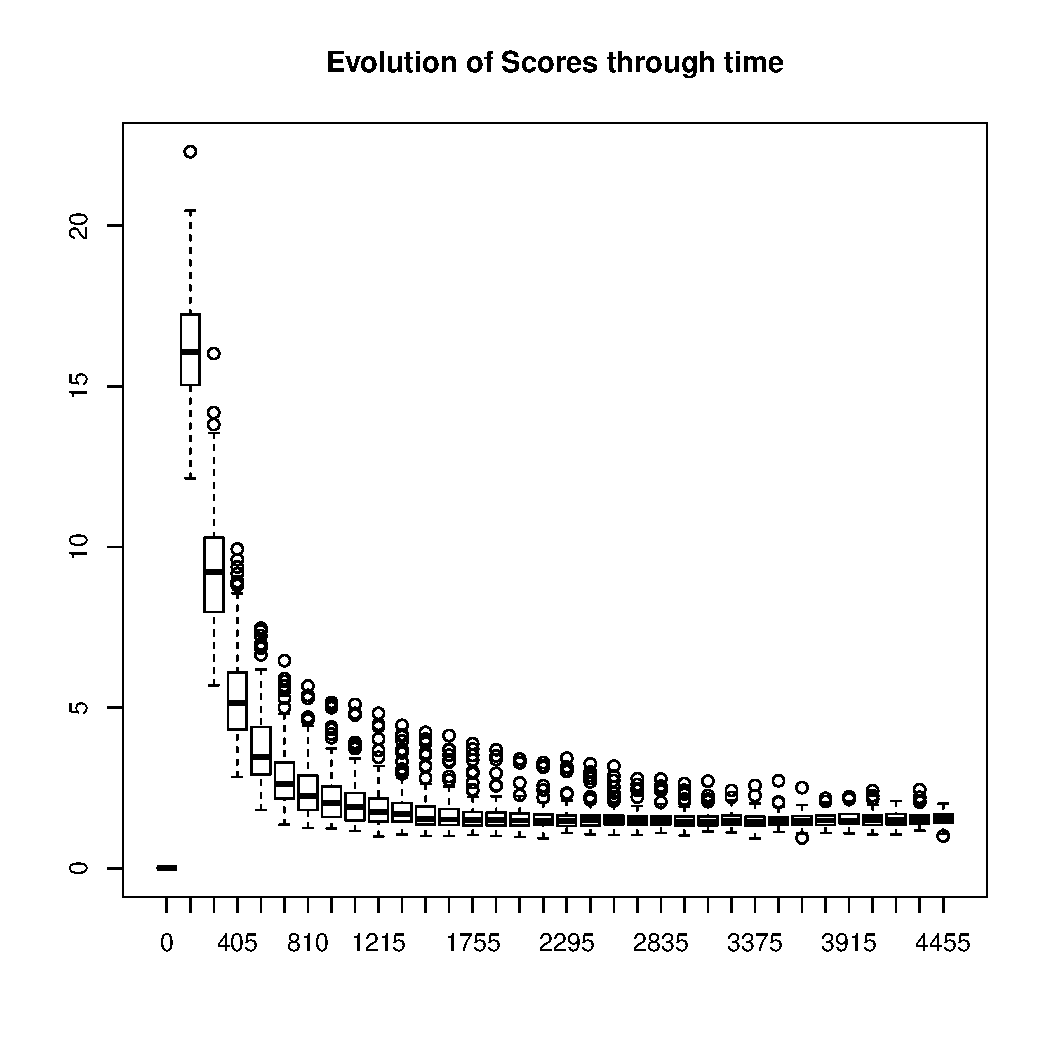
\includegraphics[width=.08\textwidth]{/home/scarrign/projects/PhD/doc/thesis/images/Scores-5_cult-prod_init-rand_volsel-gin_ufun-cust.pdf}	& \includegraphics[width=.08\textwidth]{/home/scarrign/projects/PhD/doc/thesis/images/Scores-3_cult-prod_init-man_volsel-gino_ufun-cust.pdf}	\\
%		&			&ginU	& 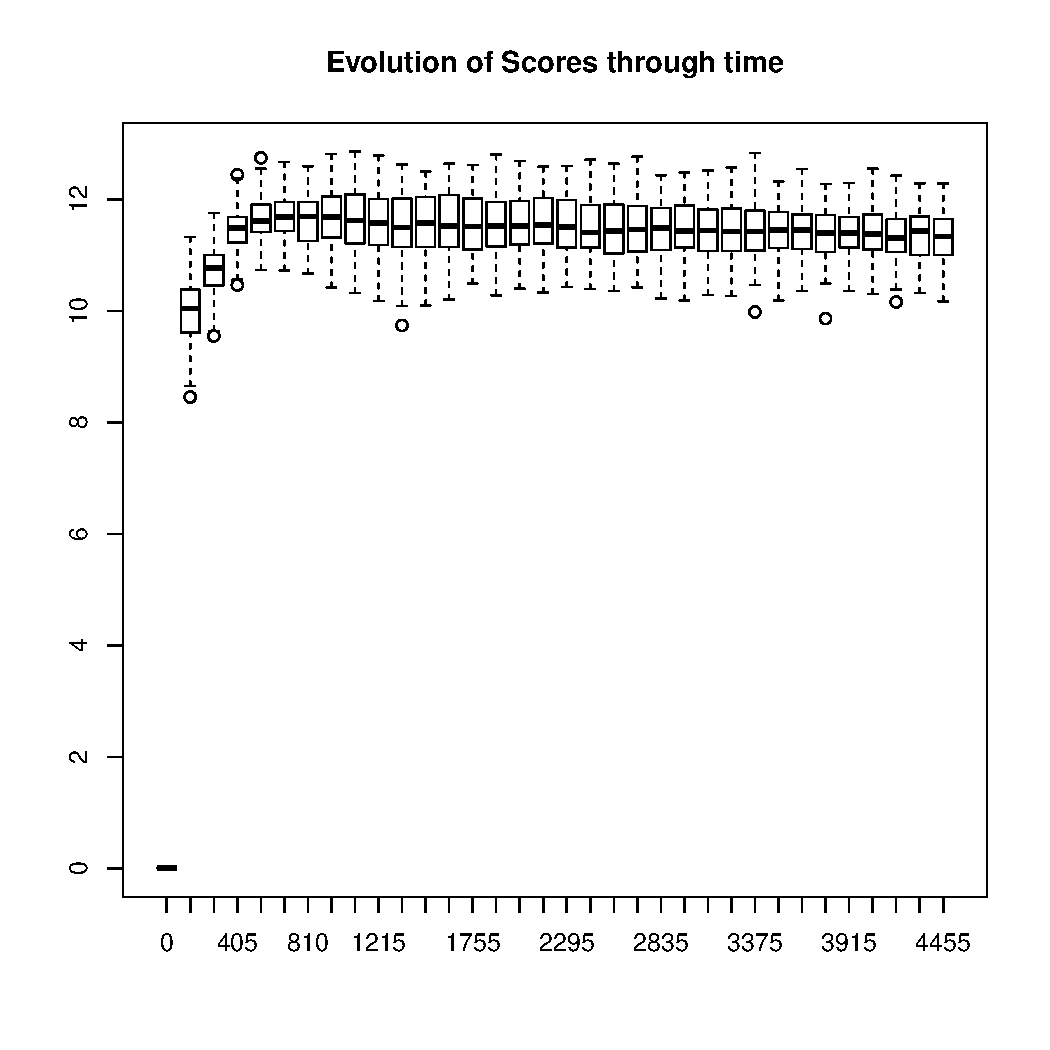
\includegraphics[width=.08\textwidth]{/home/scarrign/projects/PhD/doc/thesis/images/Scores-4_cult-prod_init-man_volsel-gino_ufun-gin.pdf}	&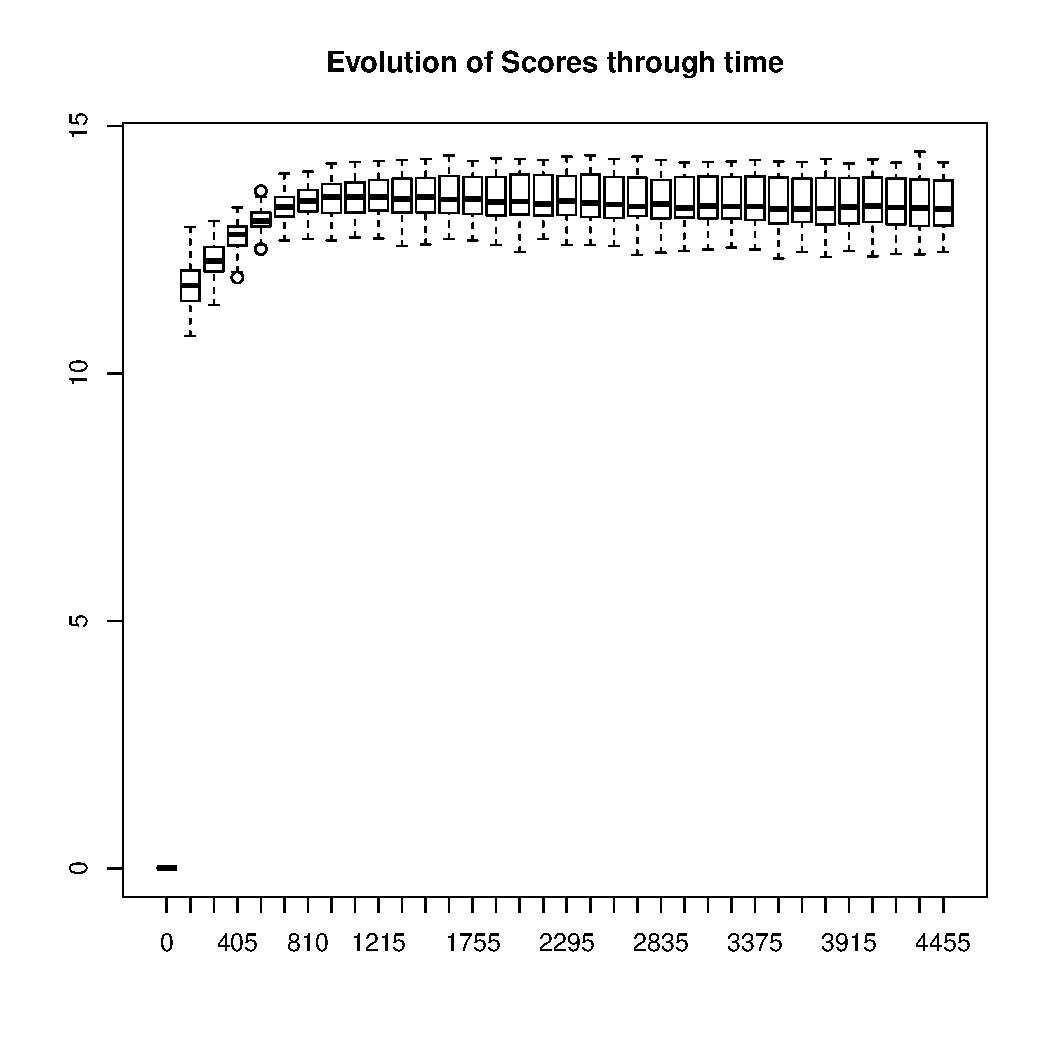
\includegraphics[width=.08\textwidth]{/home/scarrign/projects/PhD/doc/thesis/images/Scores-2_cult-prod_init-man_volsel-gin_ufun-gin.pdf} 	& \includegraphics[width=.08\textwidth]{/home/scarrign/projects/PhD/doc/thesis/images/Scores-6_cult-prod_init-rand_volsel-gin_ufun-gin.pdf}	\\
%		&\multirow{2}{*}{cust}	&cust	& \includegraphics[width=.08\textwidth]{/home/scarrign/projects/PhD/doc/thesis/images/Scores-7_cult-prod_init-rand_volsel-gino_ufun-cust.pdf}	& \includegraphics[width=.08\textwidth]{/home/scarrign/projects/PhD/doc/thesis/images/Scores-8_cult-prod_init-rand_volsel-gino_ufun-gin.pdf}	& 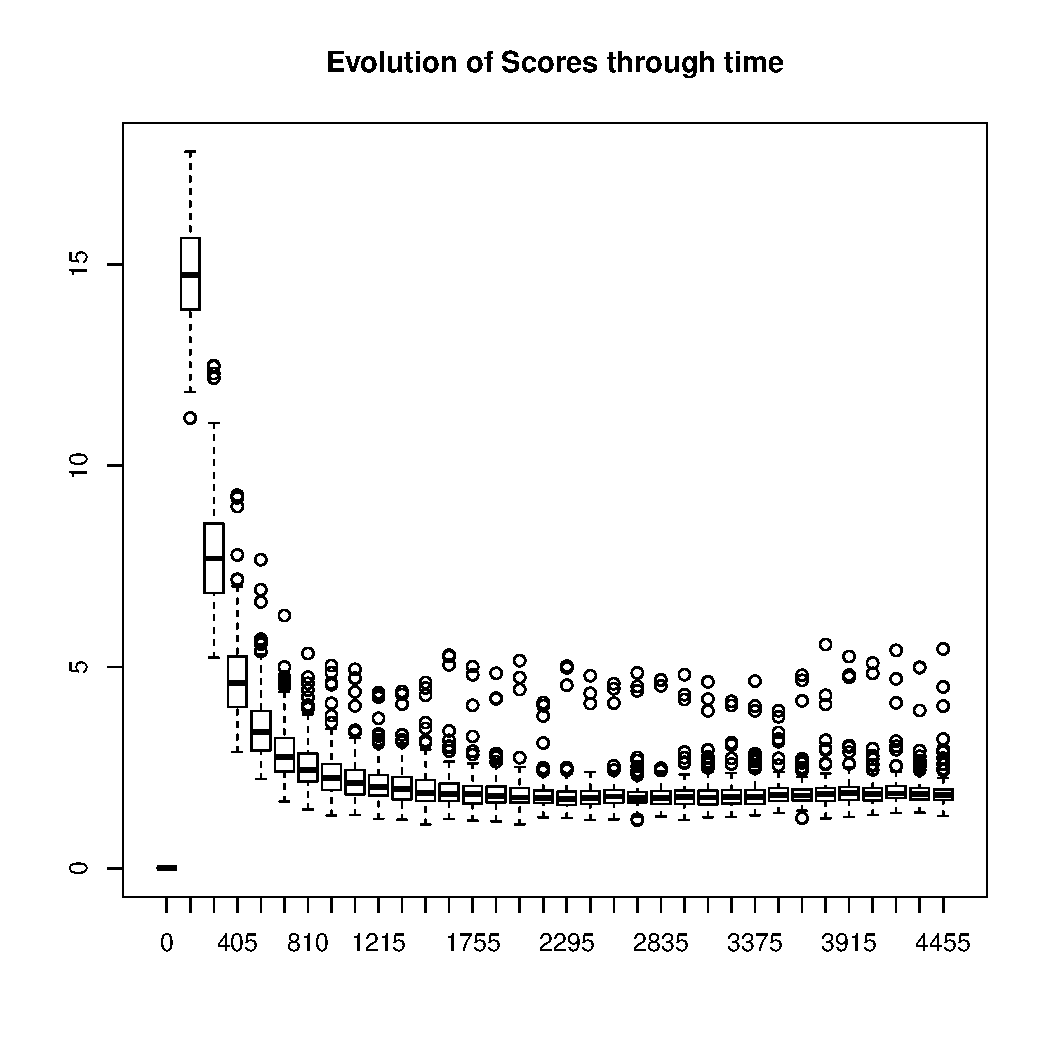
\includegraphics[width=.08\textwidth]{/home/scarrign/projects/PhD/doc/thesis/images/Scores-9_cult-prod_init-randn_volsel-gin_ufun-cust.pdf}	\\
%		&			&ginU	& \includegraphics[width=.08\textwidth]{/home/scarrign/projects/PhD/doc/thesis/images/Scores-10_cult-prod_init-randn_volsel-gin_ufun-gin.pdf}	& \includegraphics[width=.08\textwidth]{/home/scarrign/projects/PhD/doc/thesis/images/Scores-11_cult-prod_init-randn_volsel-gino_ufun-cust.pdf}	& 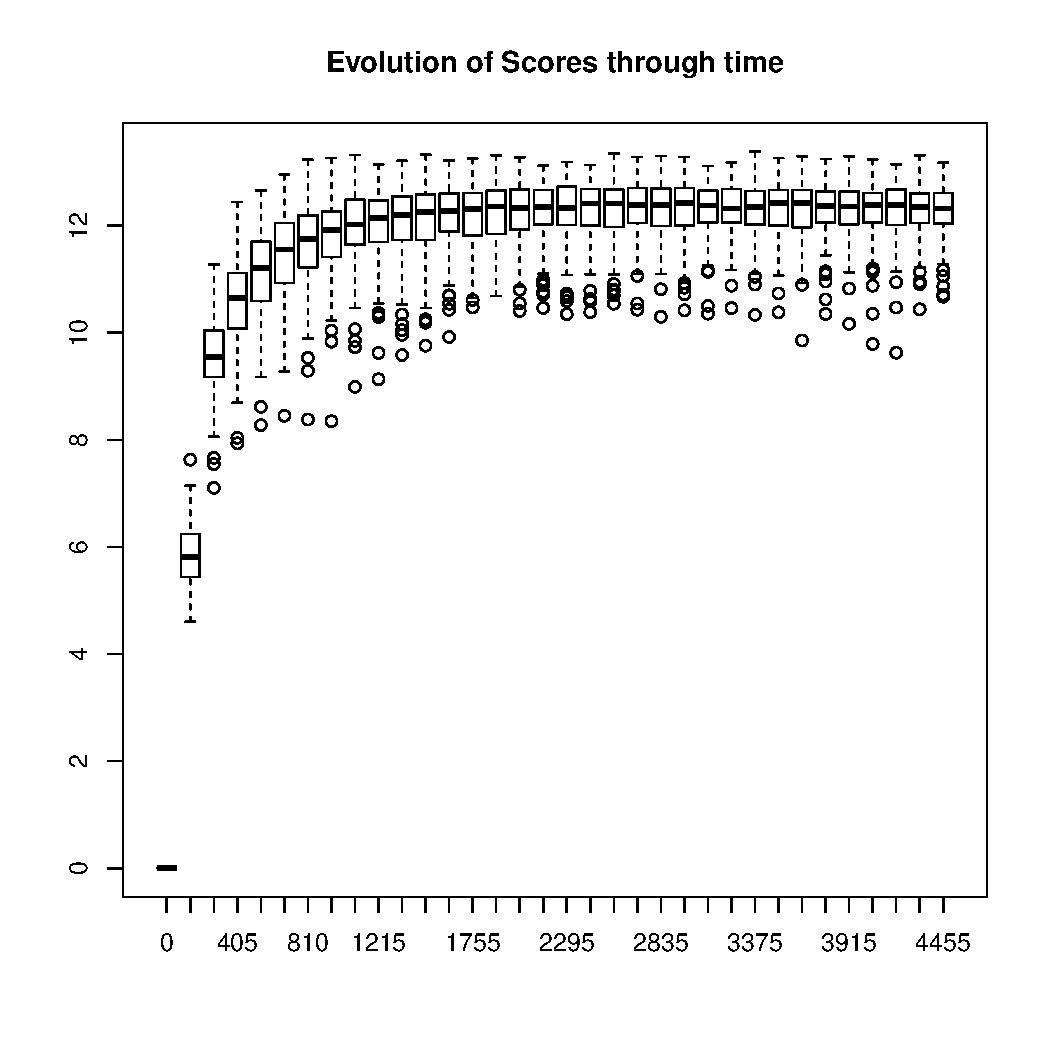
\includegraphics[width=.08\textwidth]{/home/scarrign/projects/PhD/doc/thesis/images/Scores-12_cult-prod_init-randn_volsel-gino_ufun-gin.pdf}	\\
%		\multirow{4}{*}{Full}	&\multirow{2}{*}{gins}	&cust	& 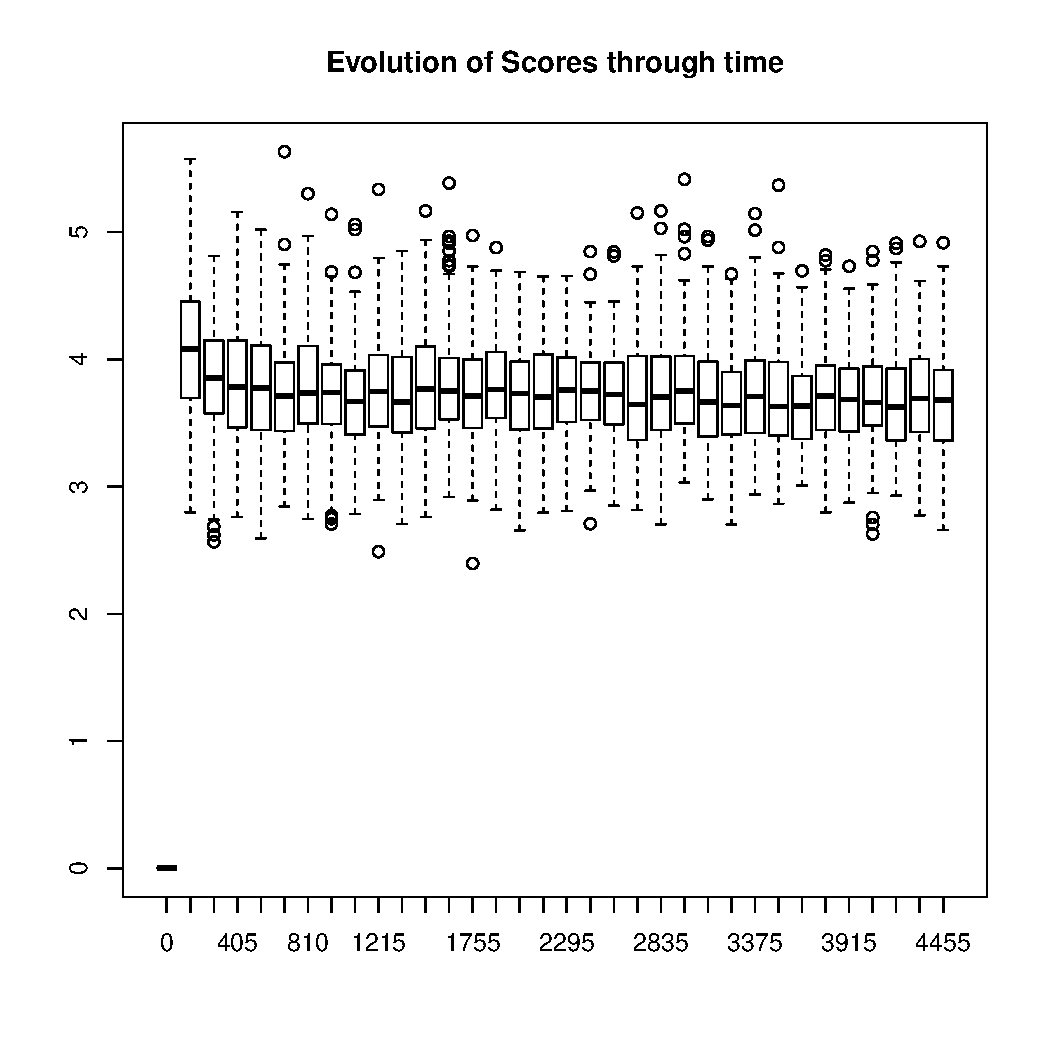
\includegraphics[width=.08\textwidth]{/home/scarrign/projects/PhD/doc/thesis/images/Scores-13_cult-integ_init-man_volsel-gin_ufun-cust.pdf}	& \includegraphics[width=.08\textwidth]{/home/scarrign/projects/PhD/doc/thesis/images/Scores-14_cult-integ_init-man_volsel-gin_ufun-gin.pdf} & 
\includegraphics[width=.08\textwidth]{/home/scarrign/projects/PhD/doc/thesis/images/Scores-15_cult-integ_init-man_volsel-gino_ufun-cust.pdf}	\\
%		    &			&ginU	& 
\includegraphics[width=.08\textwidth]{/home/scarrign/projects/PhD/doc/thesis/images/Scores-16_cult-integ_init-man_volsel-gino_ufun-gin.pdf}	& 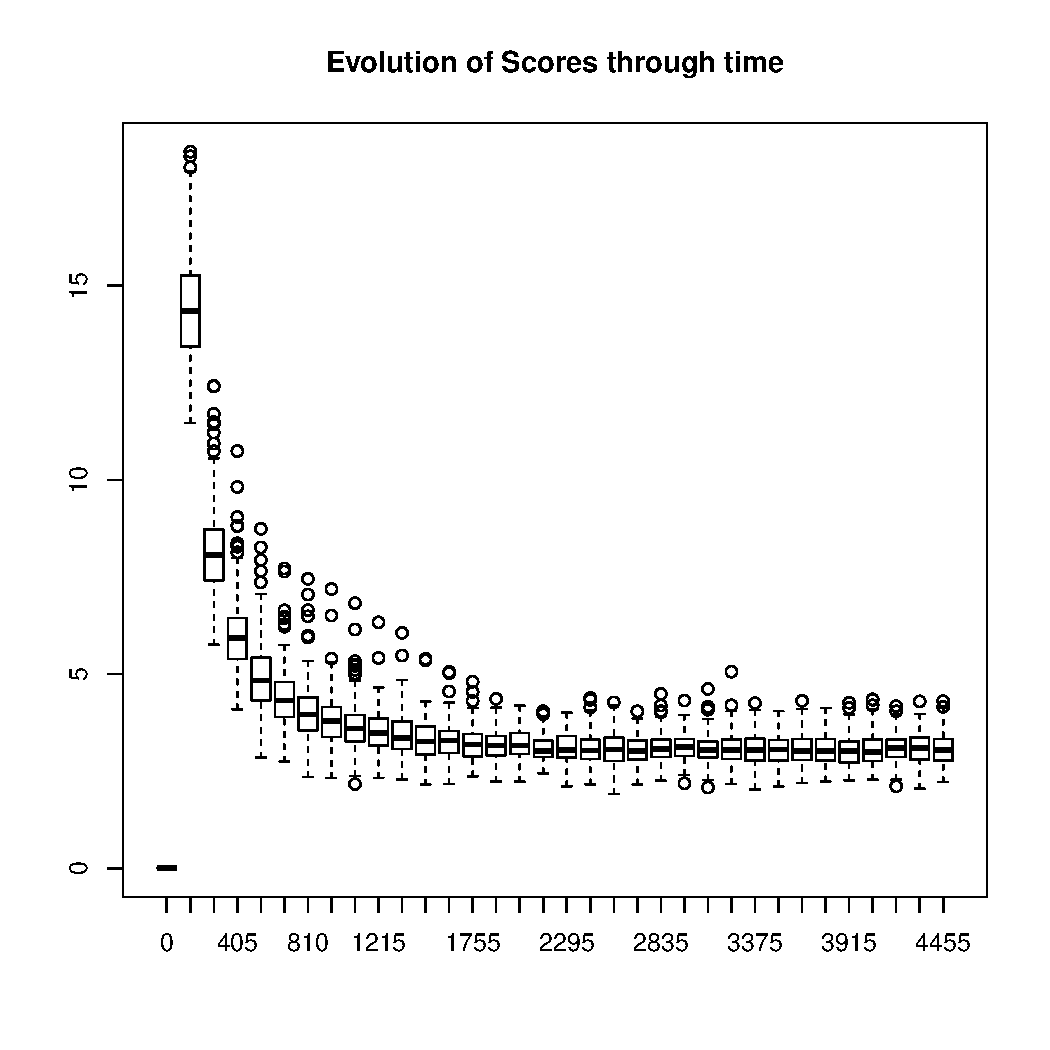
\includegraphics[width=.08\textwidth]{/home/scarrign/projects/PhD/doc/thesis/images/Scores-17_cult-integ_init-rand_volsel-gin_ufun-cust.pdf}	& \includegraphics[width=.08\textwidth]{/home/scarrign/projects/PhD/doc/thesis/images/Scores-18_cult-integ_init-rand_volsel-gin_ufun-gin.pdf}	\\
%		    &\multirow{2}{*}{cust}	&cust	& 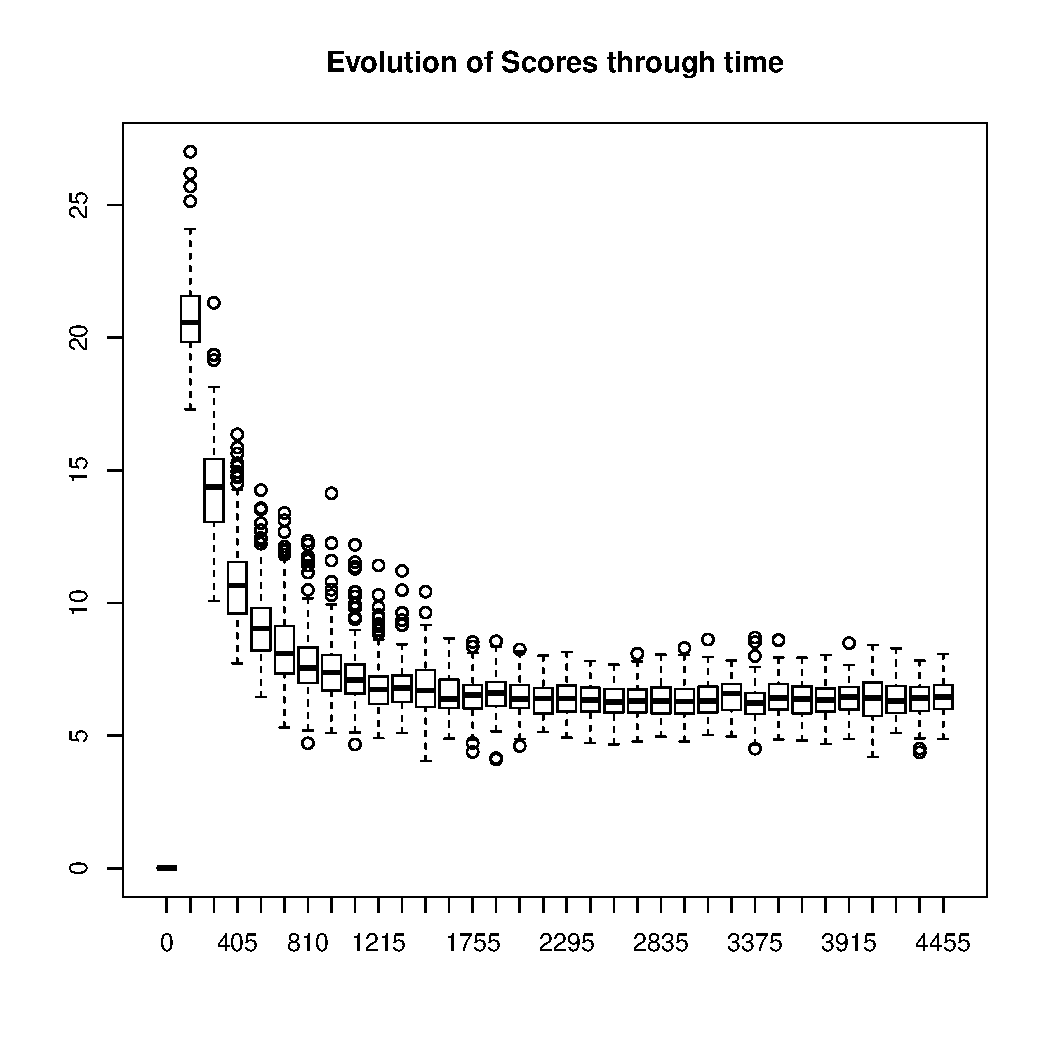
\includegraphics[width=.08\textwidth]{/home/scarrign/projects/PhD/doc/thesis/images/Scores-19_cult-integ_init-rand_volsel-gino_ufun-cust.pdf}	& 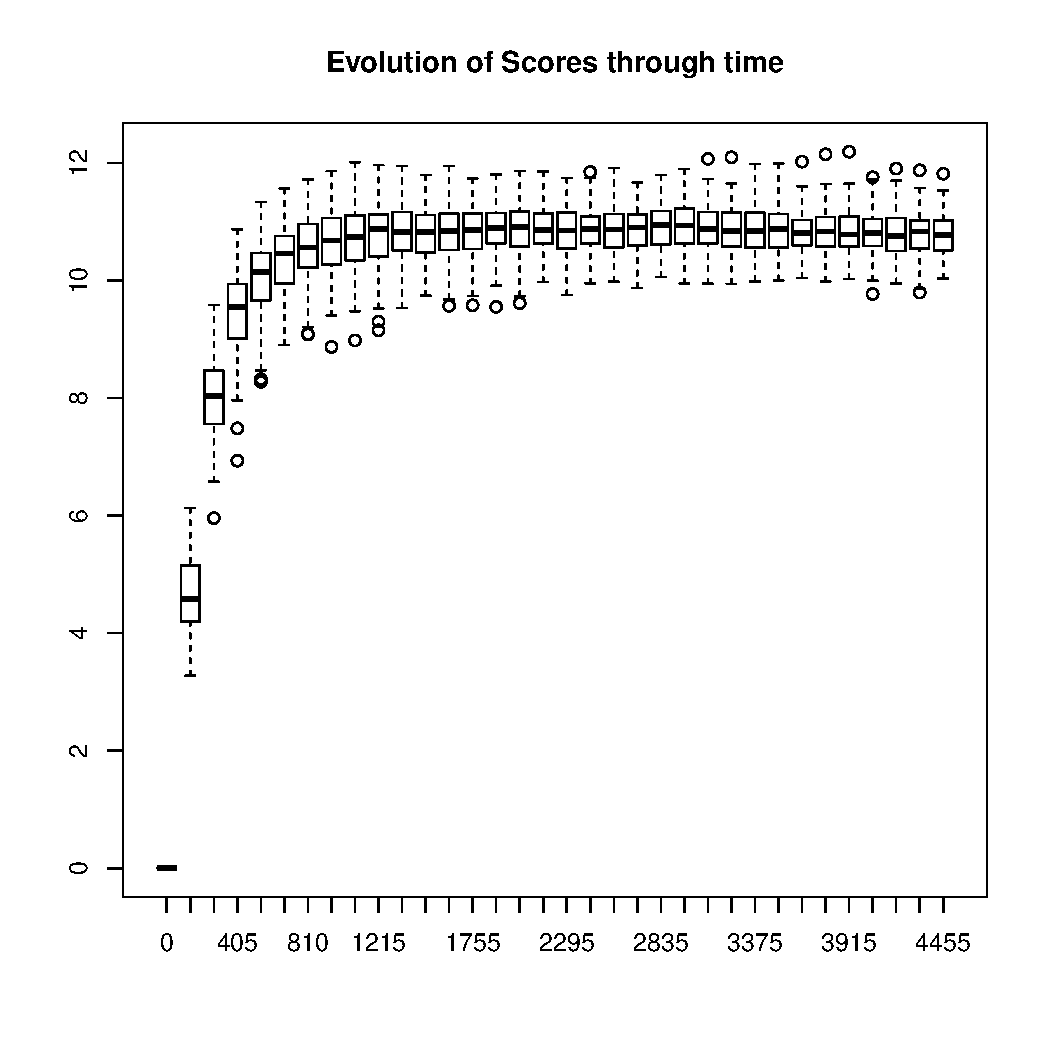
\includegraphics[width=.08\textwidth]{/home/scarrign/projects/PhD/doc/thesis/images/Scores-20_cult-integ_init-rand_volsel-gino_ufun-gin.pdf}	& \includegraphics[width=.08\textwidth]{/home/scarrign/projects/PhD/doc/thesis/images/Scores-21_cult-integ_init-randn_volsel-gin_ufun-cust.pdf}	\\
%		    &			&ginU	& 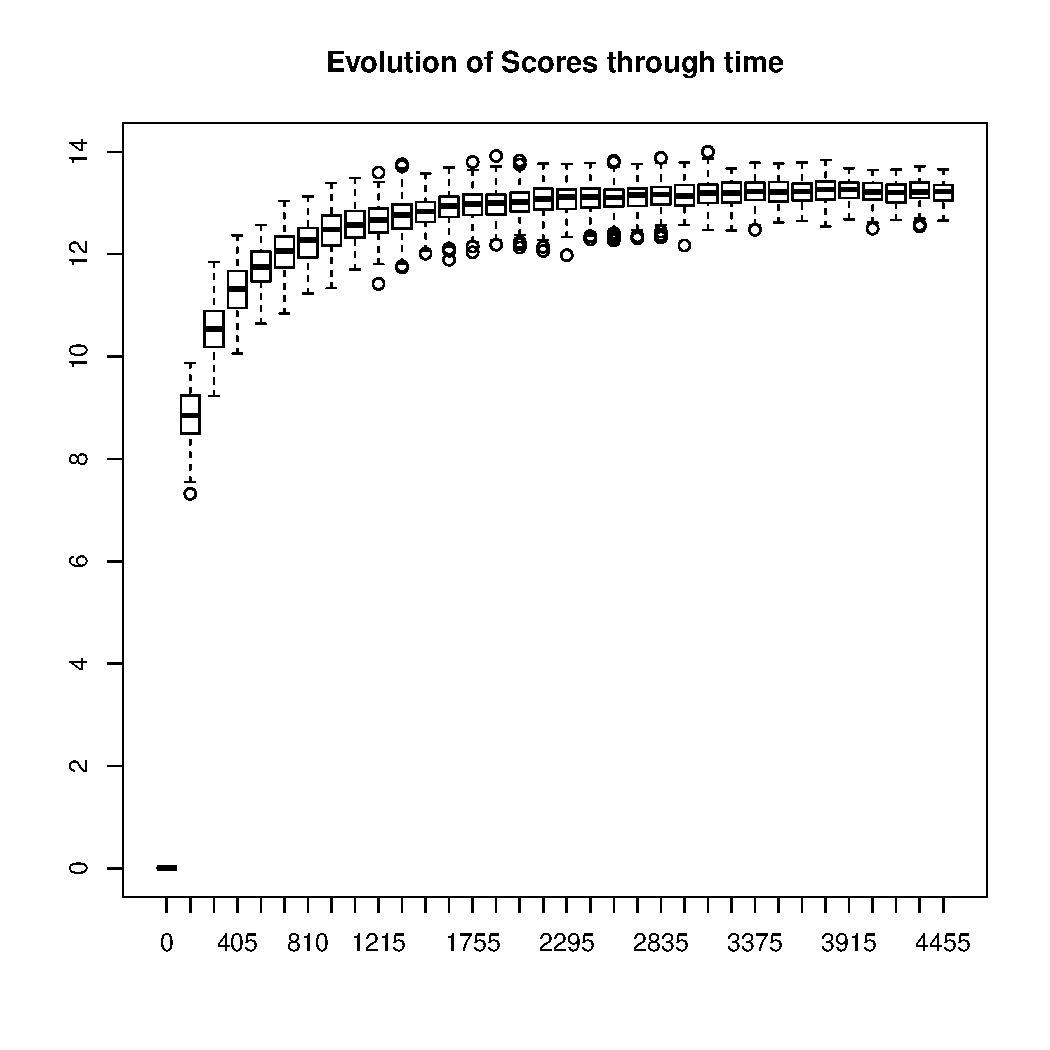
\includegraphics[width=.08\textwidth]{/home/scarrign/projects/PhD/doc/thesis/images/Scores-22_cult-integ_init-randn_volsel-gin_ufun-gin.pdf}	& 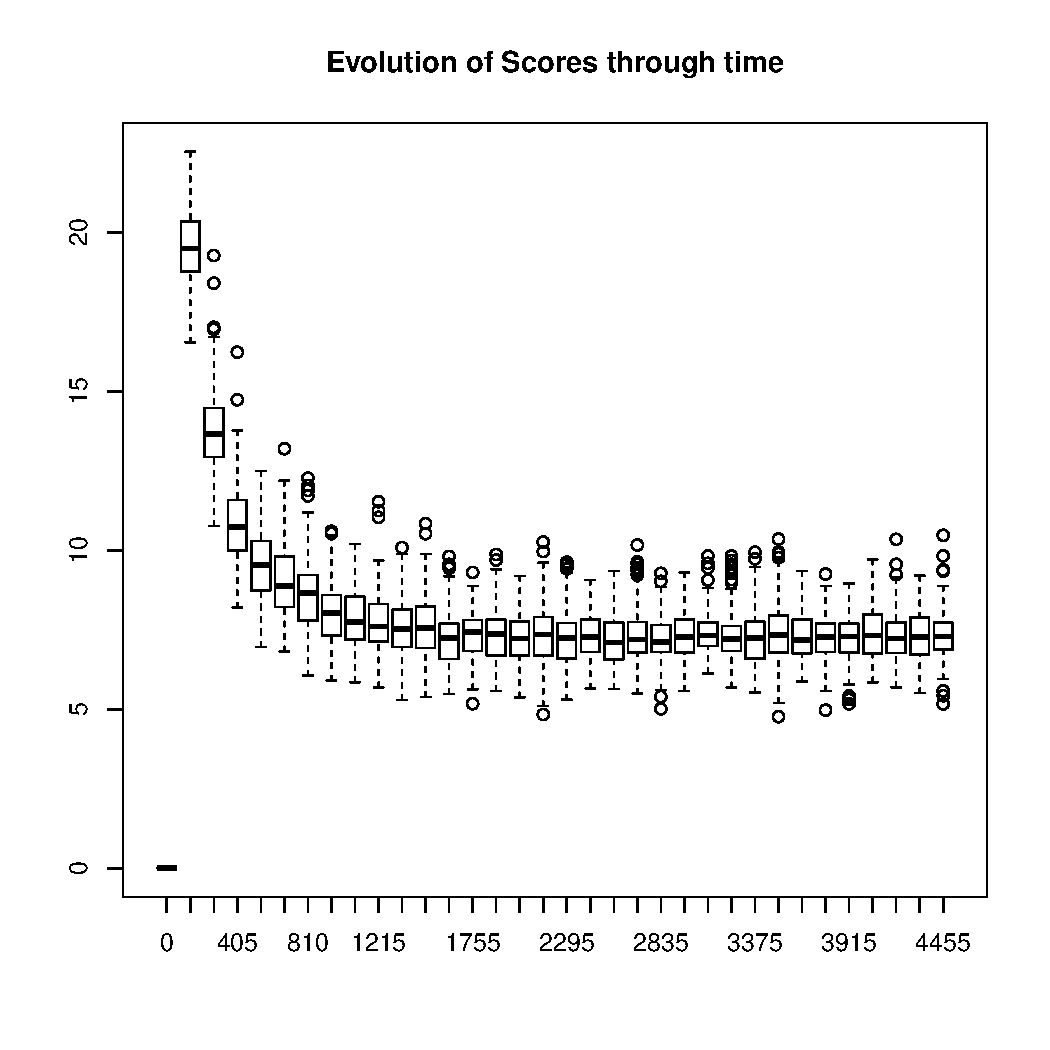
\includegraphics[width=.08\textwidth]{/home/scarrign/projects/PhD/doc/thesis/images/Scores-23_cult-integ_init-randn_volsel-gino_ufun-cust.pdf}	& \includegraphics[width=.08\textwidth]{/home/scarrign/projects/PhD/doc/thesis/images/Scores-24_cult-integ_init-randn_volsel-gino_ufun-gin.pdf}	\\
%	    
%	\end{tabular}
%    \end{table}
%\end{frame}
%
%\begin{frame}{Equilbrium indicators}
%    Evolution of Prices
%
%    \begin{table}
%	\centering
%	
%	\tiny
%	\begin{tabular}{lllccc}
%	    Copy 			& Q. Sel. 		& Util. &  \multicolumn{3}{c}{Init.}  \\
%	    				&			&	&rand	& randn & man	\\
%					\multirow{4}{*}{Full}	&\multirow{2}{*}{ginS}	& cust	& 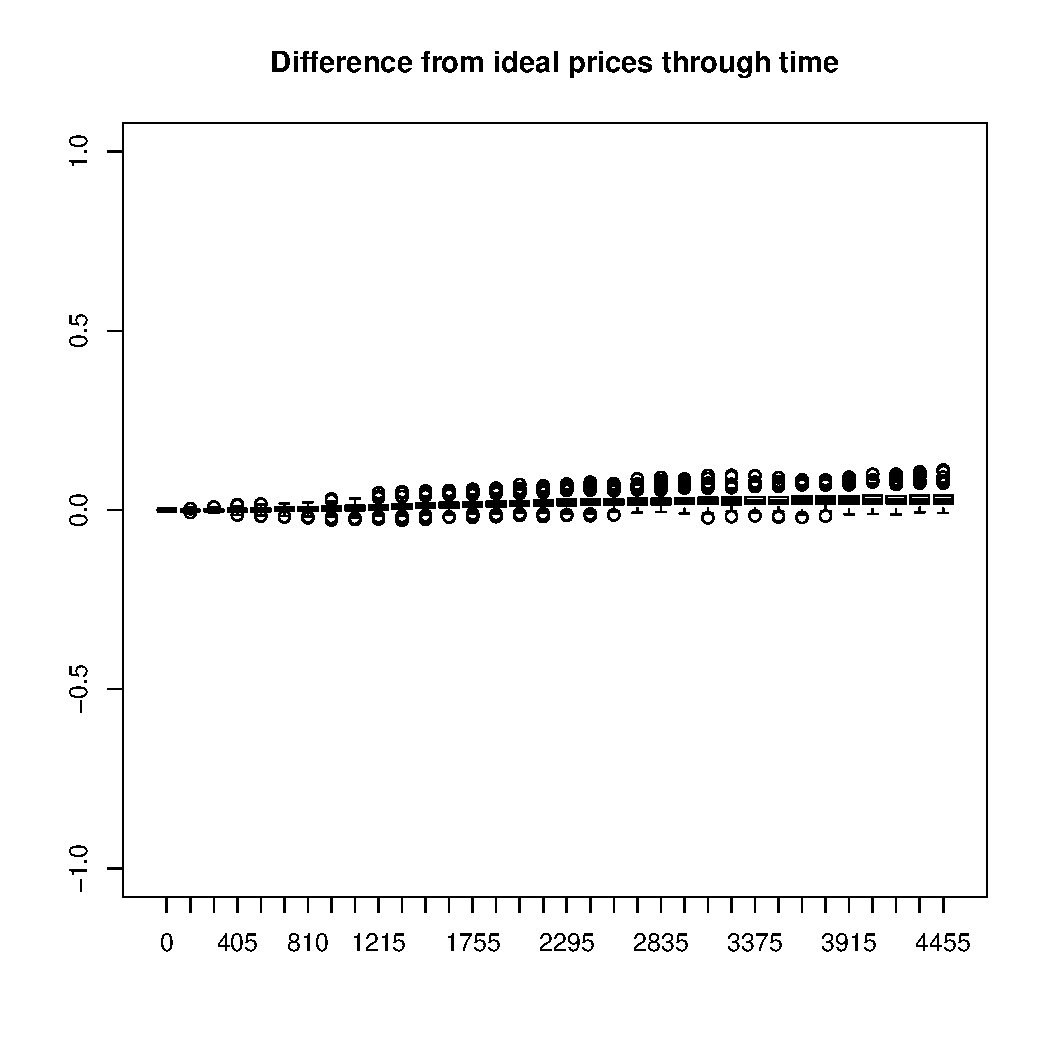
\includegraphics[width=.08\textwidth]{/home/scarrign/projects/PhD/doc/thesis/images/Prices-1_cult-prod_init-man_volsel-gin_ufun-cust.pdf}& \includegraphics[width=.08\textwidth]{/home/scarrign/projects/PhD/doc/thesis/images/Prices-5_cult-prod_init-rand_volsel-gin_ufun-cust.pdf}	& 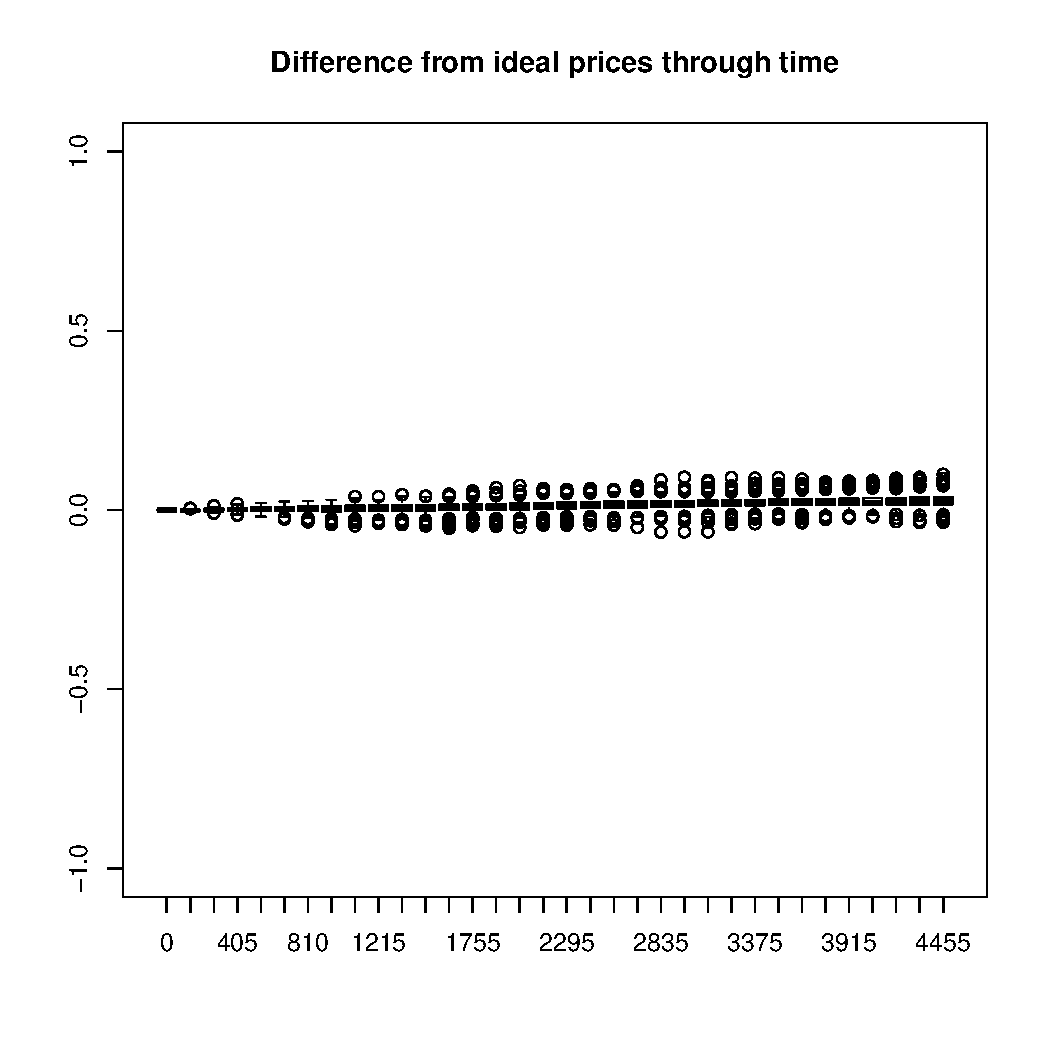
\includegraphics[width=.08\textwidth]{/home/scarrign/projects/PhD/doc/thesis/images/Prices-3_cult-prod_init-man_volsel-gino_ufun-cust.pdf}	\\
%		&			&ginU	& \includegraphics[width=.08\textwidth]{/home/scarrign/projects/PhD/doc/thesis/images/Prices-4_cult-prod_init-man_volsel-gino_ufun-gin.pdf}	&\includegraphics[width=.08\textwidth]{/home/scarrign/projects/PhD/doc/thesis/images/Prices-2_cult-prod_init-man_volsel-gin_ufun-gin.pdf} 	& \includegraphics[width=.08\textwidth]{/home/scarrign/projects/PhD/doc/thesis/images/Prices-6_cult-prod_init-rand_volsel-gin_ufun-gin.pdf}	\\
%		&\multirow{2}{*}{cust}	&cust	& \includegraphics[width=.08\textwidth]{/home/scarrign/projects/PhD/doc/thesis/images/Prices-7_cult-prod_init-rand_volsel-gino_ufun-cust.pdf}	& 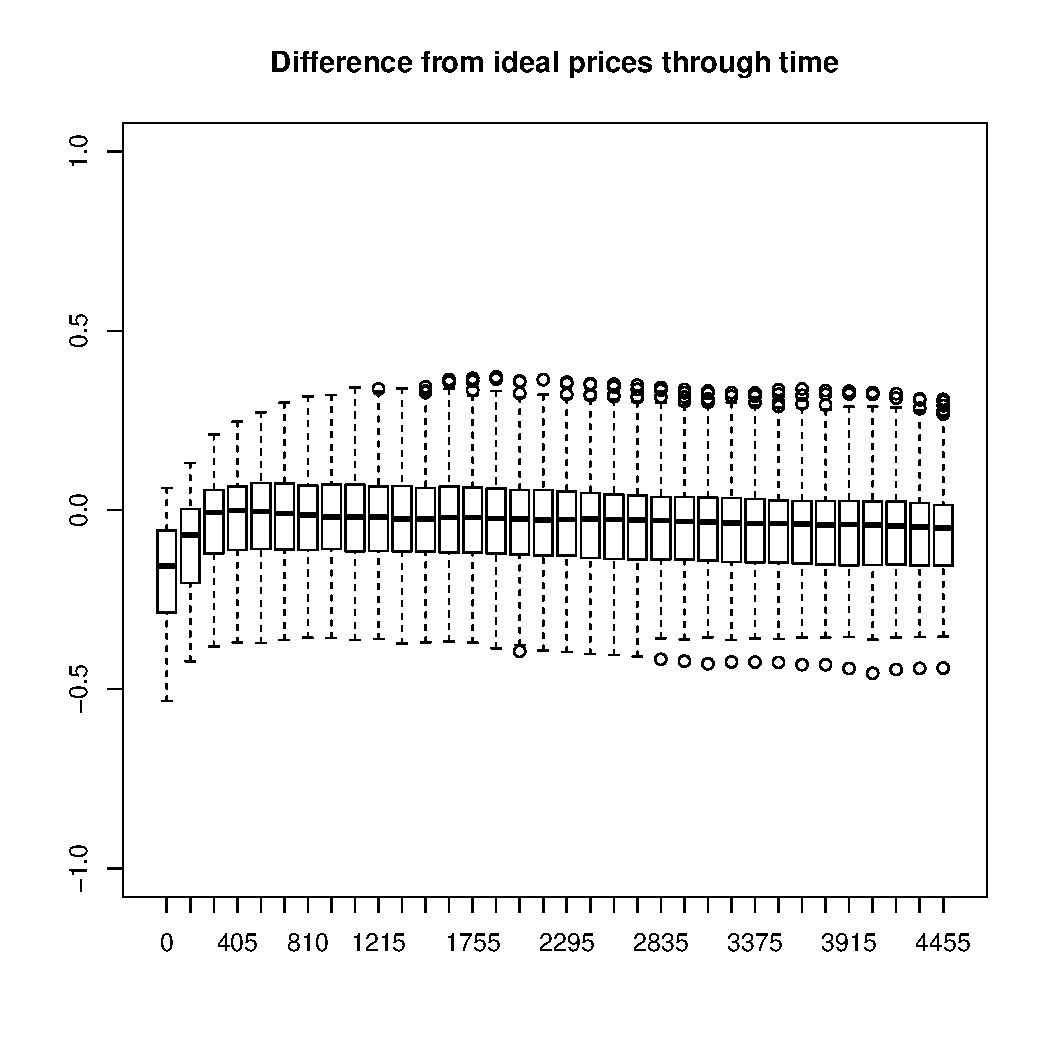
\includegraphics[width=.08\textwidth]{/home/scarrign/projects/PhD/doc/thesis/images/Prices-8_cult-prod_init-rand_volsel-gino_ufun-gin.pdf}	& \includegraphics[width=.08\textwidth]{/home/scarrign/projects/PhD/doc/thesis/images/Prices-9_cult-prod_init-randn_volsel-gin_ufun-cust.pdf}	\\
%		&			&ginU	& 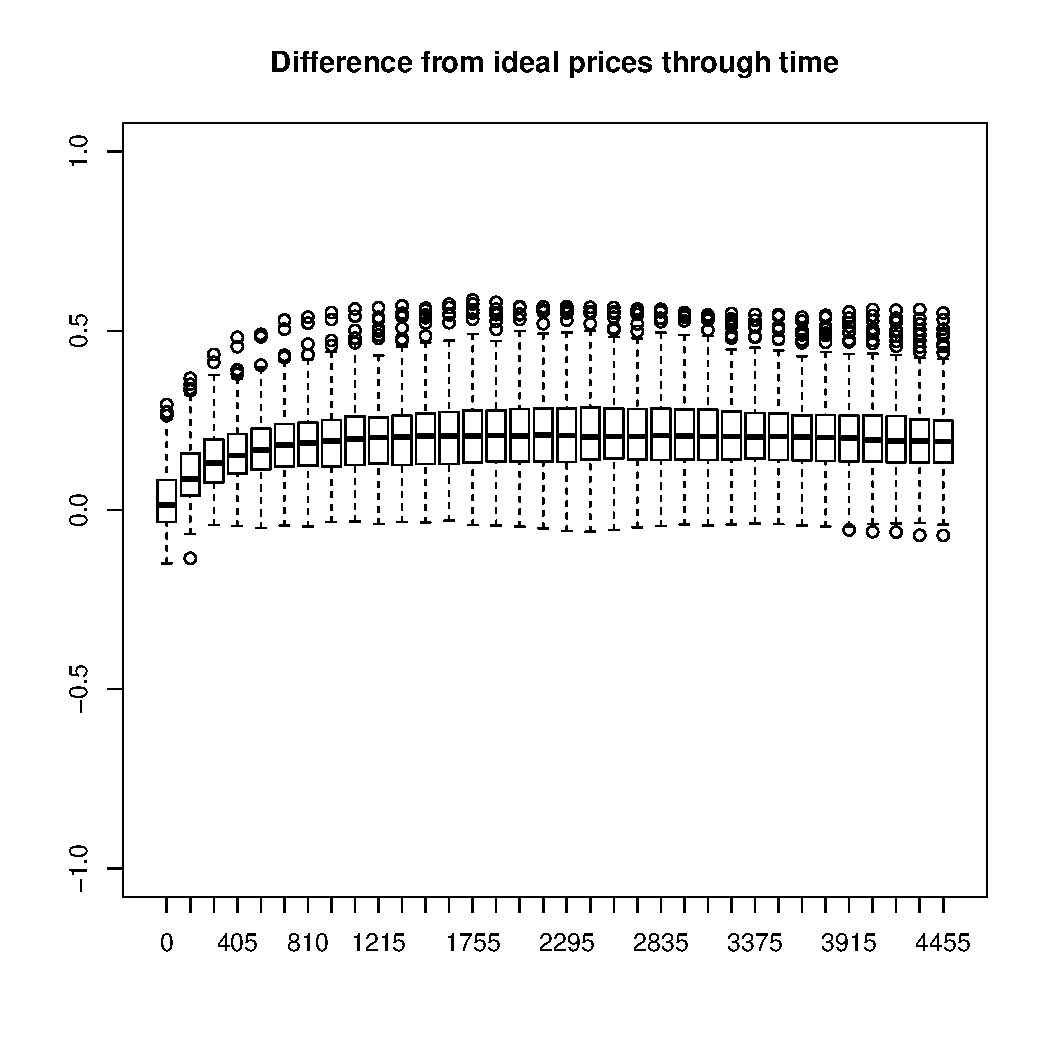
\includegraphics[width=.08\textwidth]{/home/scarrign/projects/PhD/doc/thesis/images/Prices-10_cult-prod_init-randn_volsel-gin_ufun-gin.pdf}	& 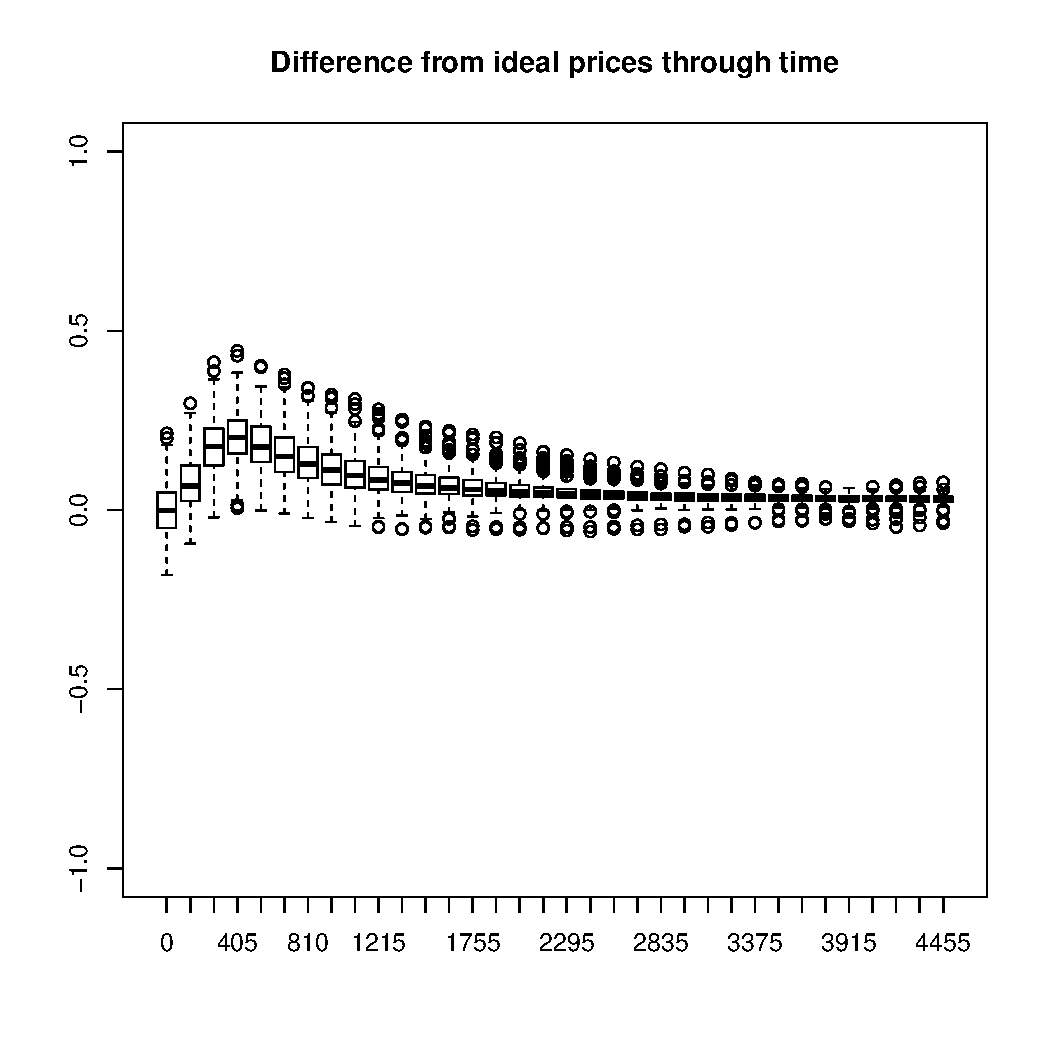
\includegraphics[width=.08\textwidth]{/home/scarrign/projects/PhD/doc/thesis/images/Prices-11_cult-prod_init-randn_volsel-gino_ufun-cust.pdf}	& 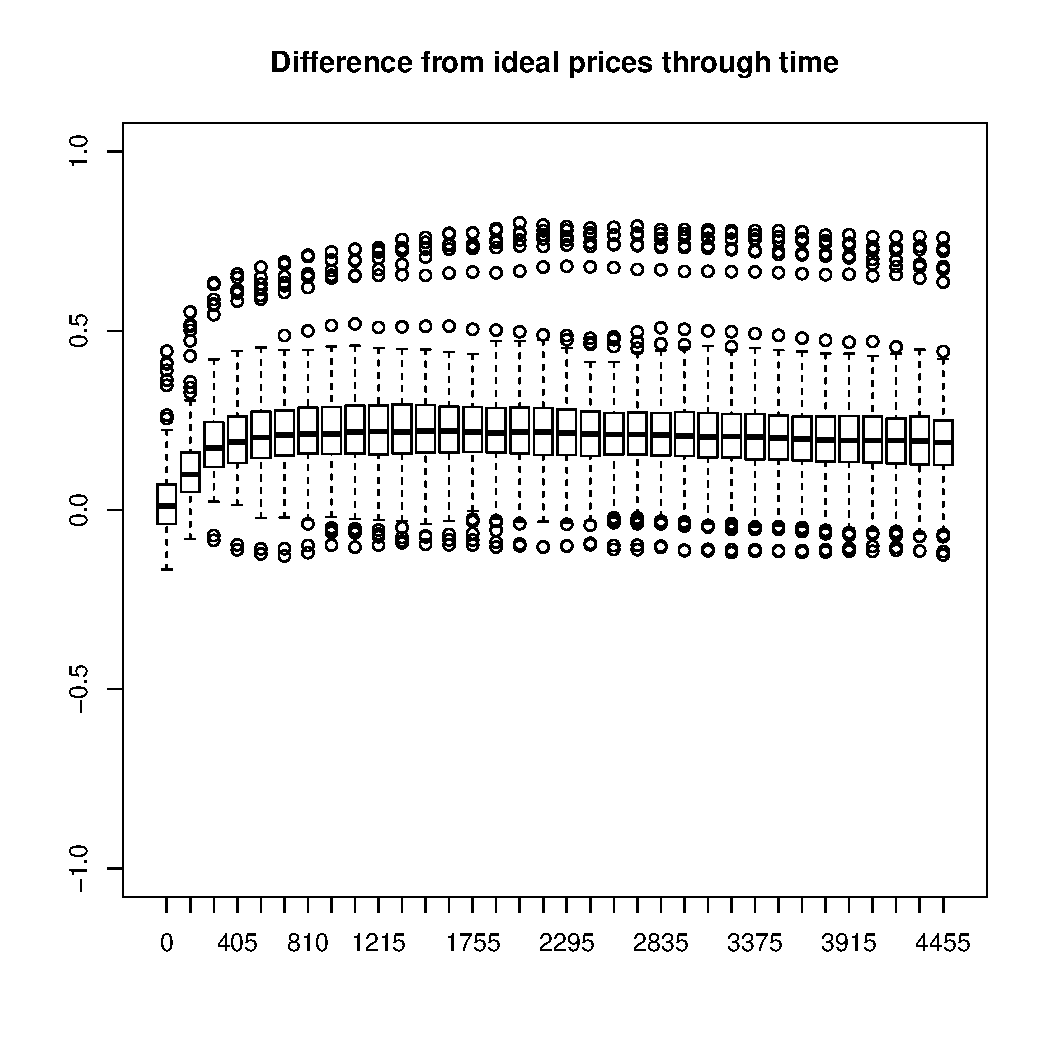
\includegraphics[width=.08\textwidth]{/home/scarrign/projects/PhD/doc/thesis/images/Prices-12_cult-prod_init-randn_volsel-gino_ufun-gin.pdf}	\\
%		\multirow{4}{*}{Full}	&\multirow{2}{*}{gins}	&cust	& 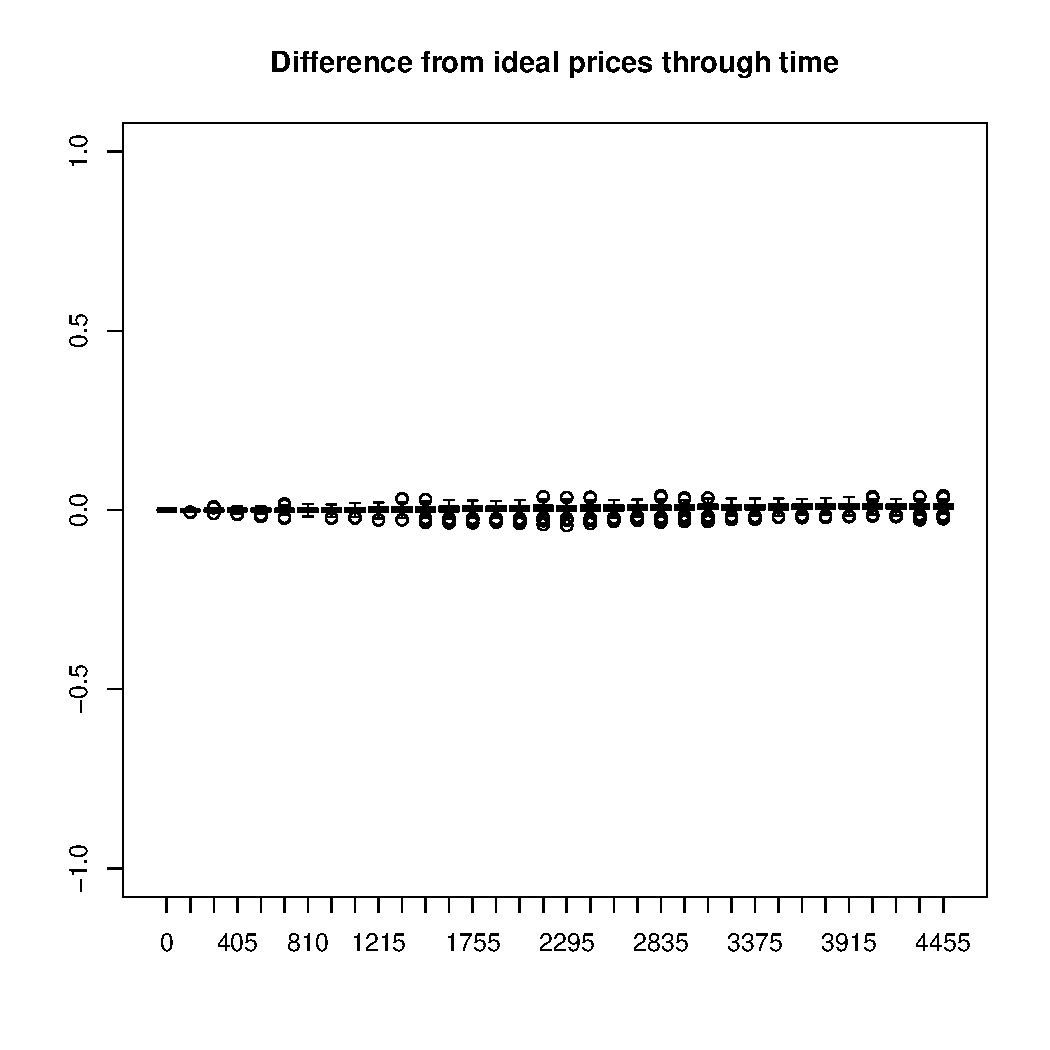
\includegraphics[width=.08\textwidth]{/home/scarrign/projects/PhD/doc/thesis/images/Prices-13_cult-integ_init-man_volsel-gin_ufun-cust.pdf}	& 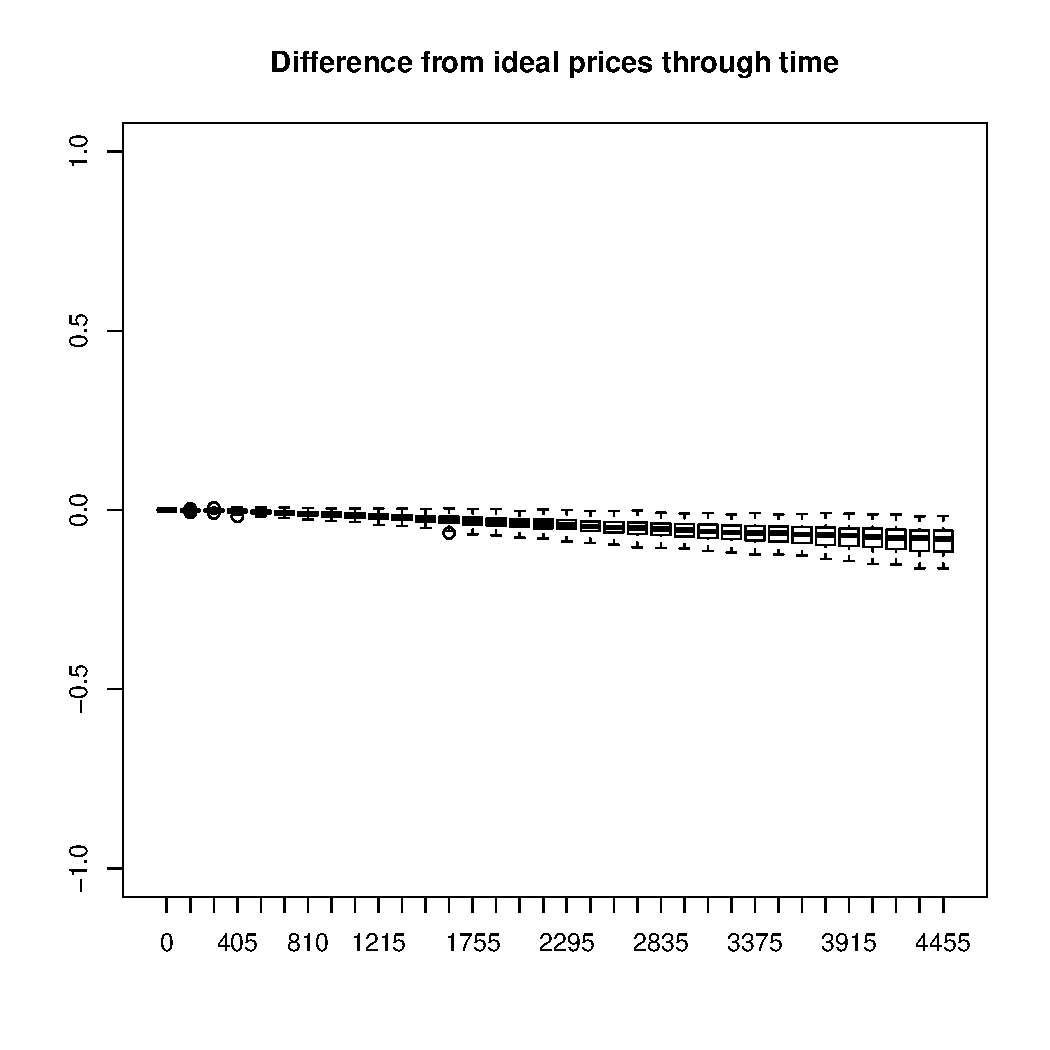
\includegraphics[width=.08\textwidth]{/home/scarrign/projects/PhD/doc/thesis/images/Prices-14_cult-integ_init-man_volsel-gin_ufun-gin.pdf} & \includegraphics[width=.08\textwidth]{/home/scarrign/projects/PhD/doc/thesis/images/Prices-15_cult-integ_init-man_volsel-gino_ufun-cust.pdf}	\\
%		    &			&ginU	& \includegraphics[width=.08\textwidth]{/home/scarrign/projects/PhD/doc/thesis/images/Prices-16_cult-integ_init-man_volsel-gino_ufun-gin.pdf}	& 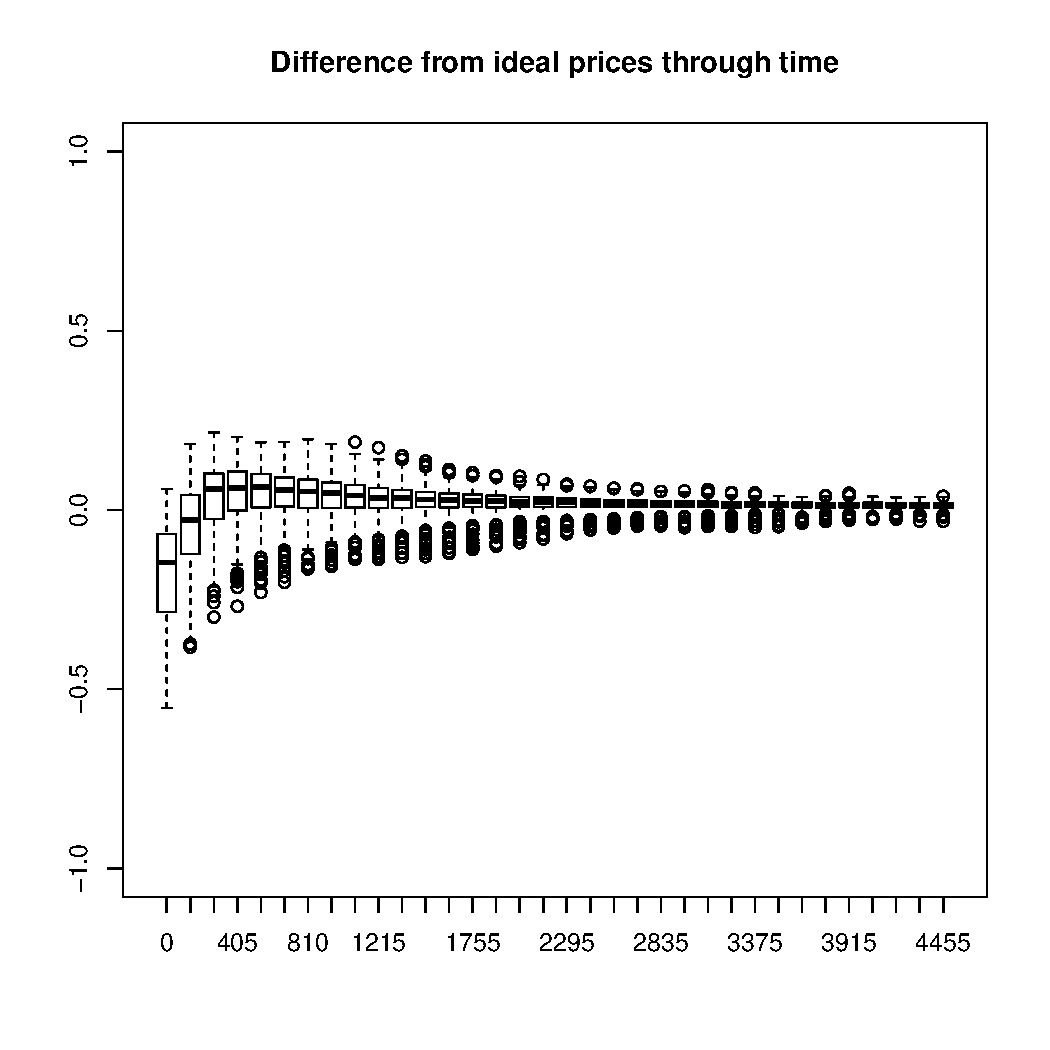
\includegraphics[width=.08\textwidth]{/home/scarrign/projects/PhD/doc/thesis/images/Prices-17_cult-integ_init-rand_volsel-gin_ufun-cust.pdf}	& \includegraphics[width=.08\textwidth]{/home/scarrign/projects/PhD/doc/thesis/images/Prices-18_cult-integ_init-rand_volsel-gin_ufun-gin.pdf}	\\
%		    &\multirow{2}{*}{cust}	&cust	& \includegraphics[width=.08\textwidth]{/home/scarrign/projects/PhD/doc/thesis/images/Prices-19_cult-integ_init-rand_volsel-gino_ufun-cust.pdf}	& 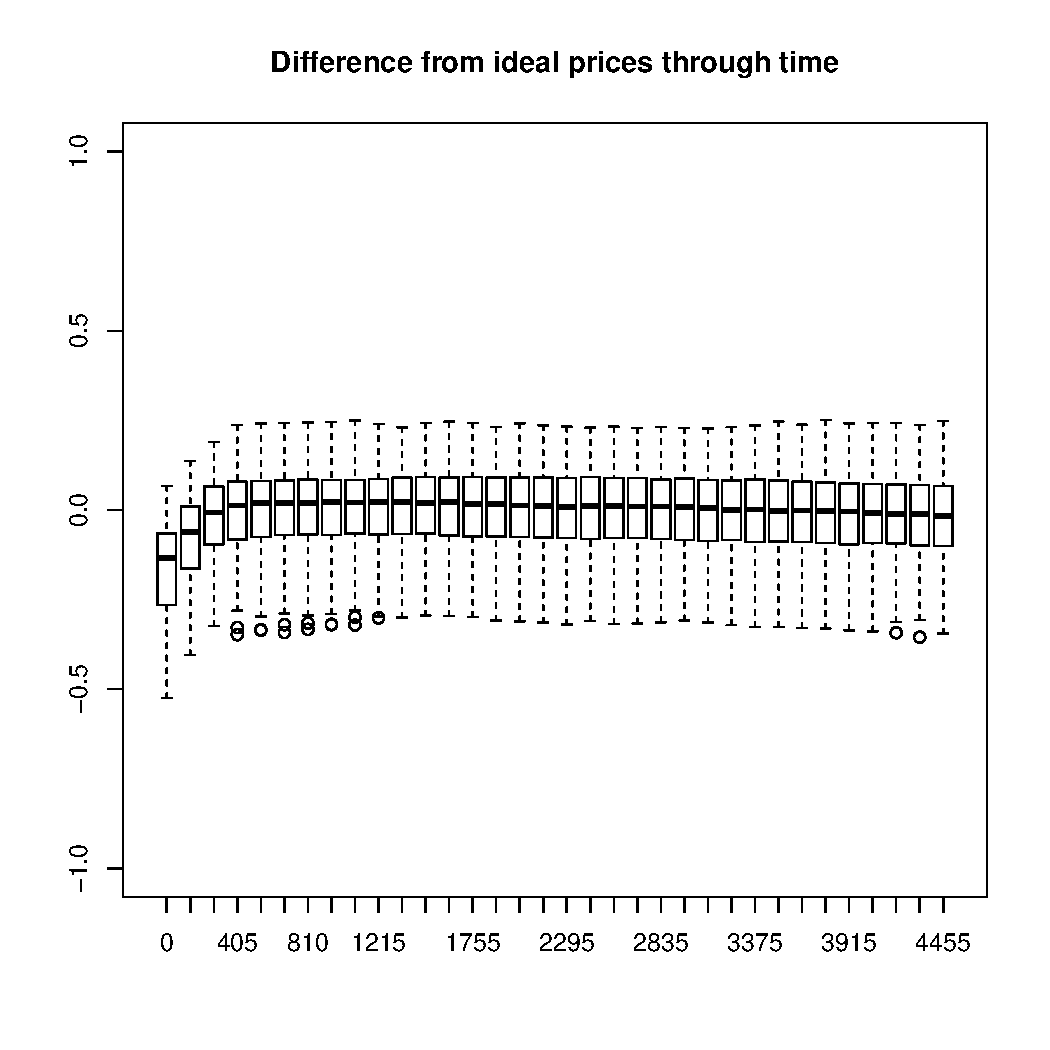
\includegraphics[width=.08\textwidth]{/home/scarrign/projects/PhD/doc/thesis/images/Prices-20_cult-integ_init-rand_volsel-gino_ufun-gin.pdf}	& \includegraphics[width=.08\textwidth]{/home/scarrign/projects/PhD/doc/thesis/images/Prices-21_cult-integ_init-randn_volsel-gin_ufun-cust.pdf}	\\
%		    &			&ginU	& 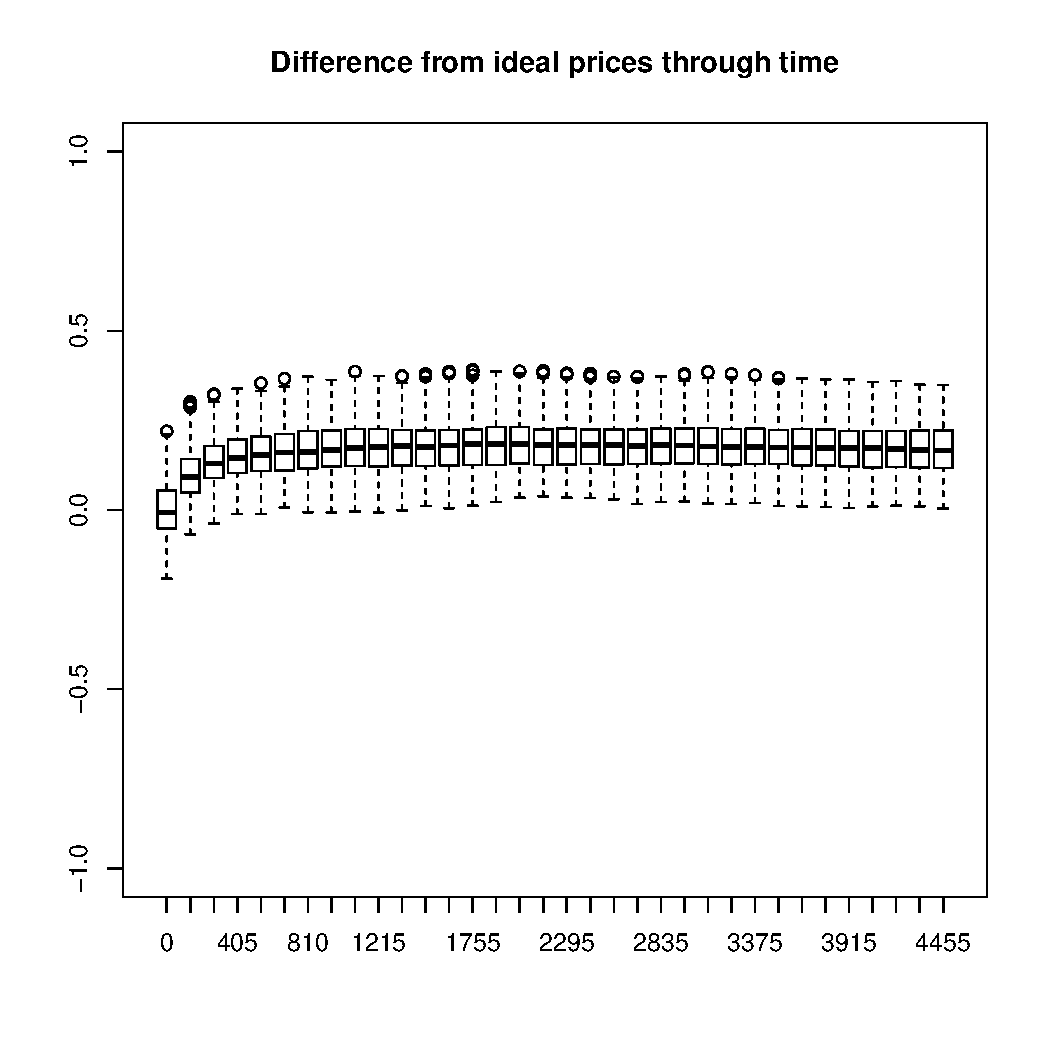
\includegraphics[width=.08\textwidth]{/home/scarrign/projects/PhD/doc/thesis/images/Prices-22_cult-integ_init-randn_volsel-gin_ufun-gin.pdf}	& \includegraphics[width=.08\textwidth]{/home/scarrign/projects/PhD/doc/thesis/images/Prices-23_cult-integ_init-randn_volsel-gino_ufun-cust.pdf}	& \includegraphics[width=.08\textwidth]{/home/scarrign/projects/PhD/doc/thesis/images/Prices-24_cult-integ_init-randn_volsel-gino_ufun-gin.pdf}	\\
%	    
%	\end{tabular}
%    \end{table}
%\end{frame}
%
%\begin{frame}{Equilbrium indicators}
%    Evolution of Quantities
%
%    \begin{table}
%	\centering
%	
%	\tiny
%	\begin{tabular}{lllccc}
%	    Copy 			& Q. Sel. 		& Util. &  \multicolumn{3}{c}{Init.}  \\
%	    				&			&	&rand	& randn & man	\\
%					\multirow{4}{*}{Full}	&\multirow{2}{*}{ginS}	& cust	& \includegraphics[width=.08\textwidth]{/home/scarrign/projects/PhD/doc/thesis/images/Quantities-1_cult-prod_init-man_volsel-gin_ufun-cust.pdf}& \includegraphics[width=.08\textwidth]{/home/scarrign/projects/PhD/doc/thesis/images/Quantities-5_cult-prod_init-rand_volsel-gin_ufun-cust.pdf}	& \includegraphics[width=.08\textwidth]{/home/scarrign/projects/PhD/doc/thesis/images/Quantities-3_cult-prod_init-man_volsel-gino_ufun-cust.pdf}	\\
%		&			&ginU	& \includegraphics[width=.08\textwidth]{/home/scarrign/projects/PhD/doc/thesis/images/Quantities-4_cult-prod_init-man_volsel-gino_ufun-gin.pdf}	&\includegraphics[width=.08\textwidth]{/home/scarrign/projects/PhD/doc/thesis/images/Quantities-2_cult-prod_init-man_volsel-gin_ufun-gin.pdf} 	& \includegraphics[width=.08\textwidth]{/home/scarrign/projects/PhD/doc/thesis/images/Quantities-6_cult-prod_init-rand_volsel-gin_ufun-gin.pdf}	\\
%		&\multirow{2}{*}{cust}	&cust	& \includegraphics[width=.08\textwidth]{/home/scarrign/projects/PhD/doc/thesis/images/Quantities-7_cult-prod_init-rand_volsel-gino_ufun-cust.pdf}	& \includegraphics[width=.08\textwidth]{/home/scarrign/projects/PhD/doc/thesis/images/Quantities-8_cult-prod_init-rand_volsel-gino_ufun-gin.pdf}	& \includegraphics[width=.08\textwidth]{/home/scarrign/projects/PhD/doc/thesis/images/Quantities-9_cult-prod_init-randn_volsel-gin_ufun-cust.pdf}	\\
%		&			&ginU	& \includegraphics[width=.08\textwidth]{/home/scarrign/projects/PhD/doc/thesis/images/Quantities-10_cult-prod_init-randn_volsel-gin_ufun-gin.pdf}	& \includegraphics[width=.08\textwidth]{/home/scarrign/projects/PhD/doc/thesis/images/Quantities-11_cult-prod_init-randn_volsel-gino_ufun-cust.pdf}	& \includegraphics[width=.08\textwidth]{/home/scarrign/projects/PhD/doc/thesis/images/Quantities-12_cult-prod_init-randn_volsel-gino_ufun-gin.pdf}	\\
%		\multirow{4}{*}{Full}	&\multirow{2}{*}{gins}	&cust	& \includegraphics[width=.08\textwidth]{/home/scarrign/projects/PhD/doc/thesis/images/Quantities-13_cult-integ_init-man_volsel-gin_ufun-cust.pdf}	& \includegraphics[width=.08\textwidth]{/home/scarrign/projects/PhD/doc/thesis/images/Quantities-14_cult-integ_init-man_volsel-gin_ufun-gin.pdf} & \includegraphics[width=.08\textwidth]{/home/scarrign/projects/PhD/doc/thesis/images/Quantities-15_cult-integ_init-man_volsel-gino_ufun-cust.pdf}	\\
%		    &			&ginU	& \includegraphics[width=.08\textwidth]{/home/scarrign/projects/PhD/doc/thesis/images/Quantities-16_cult-integ_init-man_volsel-gino_ufun-gin.pdf}	& \includegraphics[width=.08\textwidth]{/home/scarrign/projects/PhD/doc/thesis/images/Quantities-17_cult-integ_init-rand_volsel-gin_ufun-cust.pdf}	& \includegraphics[width=.08\textwidth]{/home/scarrign/projects/PhD/doc/thesis/images/Quantities-18_cult-integ_init-rand_volsel-gin_ufun-gin.pdf}	\\
%		    &\multirow{2}{*}{cust}	&cust	& \includegraphics[width=.08\textwidth]{/home/scarrign/projects/PhD/doc/thesis/images/Quantities-19_cult-integ_init-rand_volsel-gino_ufun-cust.pdf}	& \includegraphics[width=.08\textwidth]{/home/scarrign/projects/PhD/doc/thesis/images/Quantities-20_cult-integ_init-rand_volsel-gino_ufun-gin.pdf}	& \includegraphics[width=.08\textwidth]{/home/scarrign/projects/PhD/doc/thesis/images/Quantities-21_cult-integ_init-randn_volsel-gin_ufun-cust.pdf}	\\
%		    &			&ginU	& \includegraphics[width=.08\textwidth]{/home/scarrign/projects/PhD/doc/thesis/images/Quantities-22_cult-integ_init-randn_volsel-gin_ufun-gin.pdf}	& \includegraphics[width=.08\textwidth]{/home/scarrign/projects/PhD/doc/thesis/images/Quantities-23_cult-integ_init-randn_volsel-gino_ufun-cust.pdf}	& \includegraphics[width=.08\textwidth]{/home/scarrign/projects/PhD/doc/thesis/images/Quantities-24_cult-integ_init-randn_volsel-gino_ufun-gin.pdf}	\\
%	    
%	\end{tabular}
%    \end{table}
%\end{frame}


\begin{frame}{Introduction of Money}
    Actual \uncover<2->{\textcolor{green}{/Money}}
    \begin{enumerate}
	\item Production
	    \begin{itemize}
		\item <3->\textcolor{green}{Unbalanced producing: Few \emph{real good} producer, lot of ``merchant'' aka ``sites'' with money.}
	    \end{itemize}
	\item Trade
	    \begin{itemize}
		\item Select quantities \uncover<4->{\textcolor{green}{\tiny / Requested quantites depends on production}}
		\item Check ratio 
	    \end{itemize}
	\item Consumption/Fill the demand (how far from ``shopping list'')\uncover<5->{\textcolor{green}{\tiny / money is not ``consume'' \dots}}
	\item Cultural Actions \uncover<6->{\textcolor{green}{\tiny  /a priori nothing, but\dots}}
	    \begin{itemize}
		\item Copy 
		\item Inovations \uncover<7->{\textcolor{green}{\tiny / should 'value' of price evolve?}}
	    \end{itemize}
    \end{enumerate}
    
\end{frame}

\begin{frame}{}

    Then optimal 'shopping list' changes


\end{frame}
\begin{frame}{Introduction of Money}
    \begin{itemize}
	\item New good called ``coins'': $p_{coins}=1$ and coins aren't consumed (\emph{ie} they don't enter in the rating funcion)
	\item Big amount of ``coins''-producers (ie people that just receive a certain amount of money)
	\item Few producers producing and selling ``hard'' goods (1 per good following exemple)
    \end{itemize}
\end{frame}

\begin{frame}{New Good Introduciton}
    \centering
    \begin{itemize}
	    \small
	\item Long Introdution Rate \includegraphics[height=2.2cm]{/home/scarrign/projects/PhD/doc/thesis/images/checkEquilLong.pdf}\\
	\item Short Introduction Rate \includegraphics[height=2.2cm]{/home/scarrign/projects/PhD/doc/thesis/images/checkEquilShort.pdf}\\
	\item Short Introduction Rate Low $\mu$  \includegraphics[height=2.2cm]{/home/scarrign/projects/PhD/doc/thesis/images/checkEquilShortLowMu.pdf}\\
    \end{itemize}
\end{frame}

\begin{frame}{Number of site with good 'N'}
    \small
Data \hfill Long Rate \hfill Short Rate \hfill Short + low $\mu$ 
	\includegraphics[width=\textwidth]{/home/scarrign/projects/PhD/doc/thesis/images/hmNbSiteWGoodN.pdf}\\
	\includegraphics[width=\textwidth]{/home/scarrign/projects/PhD/doc/thesis/images/plotNbSiteWGoodN.pdf}\\
\end{frame}

\begin{frame}{Number of site with 'N'differents goods}
    \centering
    \tiny
Long Introdution Rate \hfill Short Rate \hfill Short + low $\mu$ 
	\includegraphics[width=.95\textwidth]{/home/scarrign/projects/PhD/doc/thesis/images/hmNbGoodPerSite.pdf}\\
	\vfil
	\includegraphics[width=.95\textwidth]{/home/scarrign/projects/PhD/doc/thesis/images/plotNbGoodPerSite.pdf}\\
\end{frame}

\begin{frame}
    Simulations with ``real'' parameters:
    \begin{itemize}
	\item 1000 agents
	\item 5 goods (+money) to appear 
	\item 200 ``cultural'' steps 
	\item 3000 ``trade'' steps ($15\times200$)
	\item every 40 cultural steps (ie $600$ trade step) a new good appears.
	\item $\approx 35min$
    \end{itemize}

\end{frame}

\begin{frame}{ Experimental framework}
    \begin{itemize}
	\item Test change in $\mu$ aka innovation rate aka ``I randomly change a price''
	\item Test change in $\lambda$, a factory to increase the probability that I'll copy someone better than me
	\item ( also $\mu$ amplitude, \emph{ie} the how much i can change the price when I decide to do so, not shown here)
    \end{itemize}
\end{frame}
\begin{frame}{Parameter tested}
    \begin{itemize}
	\item $\lambda \in \{0.0001,0.001,0.01,0.1,1,10\}$
	\item $\mu \in \{0.001,0.01,0.1,1\}$
	\item  $ 6 \times 4 = 24$ setup, 50s simulation each
    \end{itemize}
\end{frame}

\begin{frame}{Result}
    Equilibrium
    \begin{table}
	\centering
	\begin{tabular}{c m{2.5cm}c m{2.5cm}}
	    \multicolumn{2}{c}{\vspace{-1cm}\tiny Quantities at the end} &\multicolumn{2}{c}{\tiny prices at the end}\\
	    \multirow{1}{2.5cm}{\includegraphics[height=2.5cm]{/home/scarrign/projects/PhD/doc/thesis/images/QuantitieMuCopyAll.pdf}} &
	    \vspace{1cm}   \includegraphics[height=1.5cm]{/home/scarrign/projects/PhD/doc/thesis/images/QuantitieCopyAll.pdf}&
	    \multirow{1}{2.5cm}{\includegraphics[height=2.5cm]{/home/scarrign/projects/PhD/doc/thesis/images/PriceMuCopyAll.pdf}} &
	    \vspace{1cm} \includegraphics[height=1.5cm]{/home/scarrign/projects/PhD/doc/thesis/images/PriceCopyAll.pdf} \\
	    &	\includegraphics[height=1.5cm]{/home/scarrign/projects/PhD/doc/thesis/images/QuantitieMuAll.pdf}&	&\includegraphics[height=1.5cm]{/home/scarrign/projects/PhD/doc/thesis/images/PriceMuAll.pdf}\\
	\end{tabular}
    \end{table}
   
    \vspace{-1.5cm}

    

    \begin{table}

     \tiny Scores at the end
	\begin{tabular}{c m{2.5cm}}
	   \multirow{2}{2.5cm}{\includegraphics[height=2.5cm]{/home/scarrign/projects/PhD/doc/thesis/images/ScoreMuCopyAll.pdf}} &
	   \vspace{1cm}\includegraphics[height=1.5cm]{/home/scarrign/projects/PhD/doc/thesis/images/ScoreCopyAll.pdf}\\
	    & \includegraphics[height=1.5cm]{/home/scarrign/projects/PhD/doc/thesis/images/ScoreMuAll.pdf} \\
	\end{tabular}
    \end{table}
\end{frame}

\begin{frame}{Chen et. Al 2017:The copy mechanism}
    \begin{table}
    \centering
     \tiny Prices at the end
	\begin{tabular}{c m{2.5cm}}
	   \multirow{2}{2.5cm}{\includegraphics[height=2.5cm]{/home/scarrign/projects/PhD/doc/thesis/images/PriceMuCopyAll.pdf}} &
	   \vspace{1cm}\includegraphics[height=1.5cm]{/home/scarrign/projects/PhD/doc/thesis/images/PriceCopyAll.pdf}\\
	    & \includegraphics[height=1.5cm]{/home/scarrign/projects/PhD/doc/thesis/images/PriceMuAll.pdf} \\
	\end{tabular}
    \end{table}

    \tiny
    \textbf{ The ``intensity of choice'' ($\lambda$):}
    \begin{quote}
	\tiny
	 With higher $\lambda$'s, the agent’s choice is less random and is heavily
	 biased toward the better performing behavioral strategy; in other words, the degree of
	 exploration in which the agent engages is reduced. 
    \end{quote}
    \begin{figure}[htp]
	\begin{center}
	\begin{tabular}{m{4cm}cm{4cm}}
	   \includegraphics[height=2.5cm]{/home/scarrign/projects/PhD/doc/thesis/images/PriceCopyAll.pdf} & vs  &
	     \includegraphics[height=2cm]{/home/scarrign/projects/PhD/doc/thesis/images/chenetal_fig7.png} \\
	     \end{tabular}
	\end{center}
    \end{figure}
\end{frame}
\begin{frame}{Case study: Dynamics of changes}
    Final equilibrium state doesn't intereste us:\\

    {\centering $\rightarrow$ Dynamic of changes}

   
    \begin{itemize}
	\item Change in goods distribution
	\item Changes sites diversity
    \end{itemize}
    
\end{frame}

\begin{frame}{Impact on the dynamic of: }
    The copy probability (\emph{ie} Chen's intensity of choice)
    $$\mu = 0.001$$
    $$\lambda  in \{0.0001,0.001,0.01,0.1,1,10\}$$
    \begin{center}
	\includegraphics[height=2cm]{{{/home/scarrign/projects/PhD/doc/thesis/images/heatmap/heatMap-1_mu0.001-copy0.0001}}}
	\includegraphics[height=2cm]{{{/home/scarrign/projects/PhD/doc/thesis/images/heatmap/heatMap-2_mu0.001-copy0.001}}}
	\includegraphics[height=2cm]{{{/home/scarrign/projects/PhD/doc/thesis/images/heatmap/heatMap-3_mu0.001-copy0.01}}}
	\includegraphics[height=2cm]{{{/home/scarrign/projects/PhD/doc/thesis/images/heatmap/heatMap-4_mu0.001-copy0.1}}}
	\includegraphics[height=2cm]{{{/home/scarrign/projects/PhD/doc/thesis/images/heatmap/heatMap-5_mu0.001-copy1}}}
	\includegraphics[height=2cm]{{{/home/scarrign/projects/PhD/doc/thesis/images/heatmap/heatMap-6_mu0.001-copy10}}}
    \end{center}

    \begin{center}
	\includegraphics[height=2cm]{{{/home/scarrign/projects/PhD/doc/thesis/images/plot/plot-1_mu0.001-copy0.0001}}}
	\includegraphics[height=2cm]{{{/home/scarrign/projects/PhD/doc/thesis/images/plot/plot-2_mu0.001-copy0.001}}}
	\includegraphics[height=2cm]{{{/home/scarrign/projects/PhD/doc/thesis/images/plot/plot-3_mu0.001-copy0.01}}}
	\includegraphics[height=2cm]{{{/home/scarrign/projects/PhD/doc/thesis/images/plot/plot-4_mu0.001-copy0.1}}}
	\includegraphics[height=2cm]{{{/home/scarrign/projects/PhD/doc/thesis/images/plot/plot-5_mu0.001-copy1}}}
	\includegraphics[height=2cm]{{{/home/scarrign/projects/PhD/doc/thesis/images/plot/plot-6_mu0.001-copy10}}}
    \end{center}
\end{frame}

\begin{frame}{Impact on the dynamic of: }
    The copy probability (\emph{ie} Chen's intensity of choice)
    $$\mu = 1$$
    $$\lambda \in \{0.0001,0.001,0.01,0.1,1,10\}$$
    \begin{center}
	\includegraphics[height=2cm]{{{/home/scarrign/projects/PhD/doc/thesis/images/heatmap/heatMap-19_mu1-copy0.0001}}}
	\includegraphics[height=2cm]{{{/home/scarrign/projects/PhD/doc/thesis/images/heatmap/heatMap-20_mu1-copy0.001}}}
	\includegraphics[height=2cm]{{{/home/scarrign/projects/PhD/doc/thesis/images/heatmap/heatMap-21_mu1-copy0.01}}}
	\includegraphics[height=2cm]{{{/home/scarrign/projects/PhD/doc/thesis/images/heatmap/heatMap-22_mu1-copy0.1}}}
	\includegraphics[height=2cm]{{{/home/scarrign/projects/PhD/doc/thesis/images/heatmap/heatMap-23_mu1-copy1}}}
	\includegraphics[height=2cm]{{{/home/scarrign/projects/PhD/doc/thesis/images/heatmap/heatMap-24_mu1-copy10}}}
    \end{center}

    \begin{center}
	\includegraphics[height=2cm]{{{/home/scarrign/projects/PhD/doc/thesis/images/plot/plot-19_mu1-copy0.0001}}}
	\includegraphics[height=2cm]{{{/home/scarrign/projects/PhD/doc/thesis/images/plot/plot-20_mu1-copy0.001}}}
	\includegraphics[height=2cm]{{{/home/scarrign/projects/PhD/doc/thesis/images/plot/plot-21_mu1-copy0.01}}}
	\includegraphics[height=2cm]{{{/home/scarrign/projects/PhD/doc/thesis/images/plot/plot-22_mu1-copy0.1}}}
	\includegraphics[height=2cm]{{{/home/scarrign/projects/PhD/doc/thesis/images/plot/plot-23_mu1-copy1}}}
	\includegraphics[height=2cm]{{{/home/scarrign/projects/PhD/doc/thesis/images/plot/plot-24_mu1-copy10}}}
    \end{center}
\end{frame}

\begin{frame}{Impact on the dynamic of: }
    The mutation rate (\emph{ie} internal innovation rate, random change of a price)
    $$\mu \in \{0.001,0.01,0.1,1\}$$
    $$\lambda = 0.0001$$
    \begin{center}
	\includegraphics[height=2cm]{{{/home/scarrign/projects/PhD/doc/thesis/images/heatmap/heatMap-1_mu0.001-copy0.0001}}}
	\includegraphics[height=2cm]{{{/home/scarrign/projects/PhD/doc/thesis/images/heatmap/heatMap-7_mu0.01-copy0.0001}}}
	\includegraphics[height=2cm]{{{/home/scarrign/projects/PhD/doc/thesis/images/heatmap/heatMap-13_mu0.1-copy0.0001}}}
	\includegraphics[height=2cm]{{{/home/scarrign/projects/PhD/doc/thesis/images/heatmap/heatMap-19_mu1-copy0.0001}}}
    \end{center}

    \begin{center}
	\includegraphics[height=2cm]{{{/home/scarrign/projects/PhD/doc/thesis/images/plot/plot-1_mu0.001-copy0.0001}}}
	\includegraphics[height=2cm]{{{/home/scarrign/projects/PhD/doc/thesis/images/plot/plot-7_mu0.01-copy0.0001}}}
	\includegraphics[height=2cm]{{{/home/scarrign/projects/PhD/doc/thesis/images/plot/plot-13_mu0.1-copy0.0001}}}
	\includegraphics[height=2cm]{{{/home/scarrign/projects/PhD/doc/thesis/images/plot/plot-19_mu1-copy0.0001}}}
    \end{center}
\end{frame}

\begin{frame}{Impact on the dynamic of: }
    The mutation rate (\emph{ie} internal innovation rate, random change of a price)
    $$\mu \in \{0.001,0.01,0.1,1\}$$
    $$\lambda = 10$$
    \begin{center}
	\includegraphics[height=2cm]{{{/home/scarrign/projects/PhD/doc/thesis/images/heatmap/heatMap-6_mu0.001-copy10}}}
	\includegraphics[height=2cm]{{{/home/scarrign/projects/PhD/doc/thesis/images/heatmap/heatMap-12_mu0.01-copy10}}}
	\includegraphics[height=2cm]{{{/home/scarrign/projects/PhD/doc/thesis/images/heatmap/heatMap-18_mu0.1-copy10}}}
	\includegraphics[height=2cm]{{{/home/scarrign/projects/PhD/doc/thesis/images/heatmap/heatMap-24_mu1-copy10}}}
    \end{center}

    \begin{center}
	\includegraphics[height=2cm]{{{/home/scarrign/projects/PhD/doc/thesis/images/plot/plot-6_mu0.001-copy10}}}
	\includegraphics[height=2cm]{{{/home/scarrign/projects/PhD/doc/thesis/images/plot/plot-12_mu0.01-copy10}}}
	\includegraphics[height=2cm]{{{/home/scarrign/projects/PhD/doc/thesis/images/plot/plot-18_mu0.1-copy10}}}
	\includegraphics[height=2cm]{{{/home/scarrign/projects/PhD/doc/thesis/images/plot/plot-24_mu1-copy10}}}
    \end{center}

\end{frame}

\begin{frame}{Hidden changes}
	Mean of non normal distribution!

	Changes in the parameters change final output by changing the whole \emph{distribution}  of how the simulation ended, not by moving the mean.
	

    \end{frame}

\begin{frame}{Distribution of simulations output}
    \tiny

	\begin{table}
	    \begin{tabular}{m{2.1cm}m{2.1cm}m{2.1cm}m{2.1cm}}
		expe & general & distrib $1Goods$ & distrib $5Goods$ \\
		mu0.001-copy0.0001 & 

		\includegraphics[height=2cm]{{{/home/scarrign/projects/PhD/doc/thesis/images/plot/plot-1_mu0.001-copy0.0001}}} &
		\includegraphics[height=2cm]{{{/home/scarrign/projects/PhD/doc/thesis/images/distrib-1goods-9000timstep-exp1_mu0.001-copy0.0001}}} &
		\includegraphics[height=2cm]{{{/home/scarrign/projects/PhD/doc/thesis/images/distrib-5goods-9000timstep-exp1_mu0.001-copy0.0001}}} \\

		mu0.01-copy0.0001 & 

		\includegraphics[height=2cm]{{{/home/scarrign/projects/PhD/doc/thesis/images/plot/plot-7_mu0.01-copy0.0001}}} &
		\includegraphics[height=2cm]{{{/home/scarrign/projects/PhD/doc/thesis/images/distrib-1goods-9000timstep-exp7_mu0.01-copy0.0001}}} &
		\includegraphics[height=2cm]{{{/home/scarrign/projects/PhD/doc/thesis/images/distrib-5goods-9000timstep-exp7_mu0.01-copy0.0001}}} \\


		mu0.001-copy10 & 

		\includegraphics[height=2cm]{{{/home/scarrign/projects/PhD/doc/thesis/images/plot/plot-6_mu0.001-copy10}}} &
		\includegraphics[height=2cm]{{{/home/scarrign/projects/PhD/doc/thesis/images/distrib-1goods-9000timstep-exp6_mu0.001-copy10}}} &
		\includegraphics[height=2cm]{{{/home/scarrign/projects/PhD/doc/thesis/images/distrib-5goods-9000timstep-exp6_mu0.001-copy10}}} \\

		mu0.01-copy10 & 

		\includegraphics[height=2cm]{{{/home/scarrign/projects/PhD/doc/thesis/images/plot/plot-12_mu0.01-copy10}}} &
		\includegraphics[height=2cm]{{{/home/scarrign/projects/PhD/doc/thesis/images/distrib-1goods-9000timstep-exp12_mu0.01-copy10}}} &
		\includegraphics[height=2cm]{{{/home/scarrign/projects/PhD/doc/thesis/images/distrib-5goods-9000timstep-exp12_mu0.01-copy10}}} \\

	    \end{tabular}
	\end{table}

\end{frame}

%%\begin{frame}{Change in copy proba}
%%    $$\mu = 0.001$$
%%    $$\lambda \in \{0.0001,0.001,0.01,0.1,1,10\}$$
%%
%%    \begin{center}
%%	\includegraphics[height=2cm]{{{/home/scarrign/projects/PhD/doc/thesis/images/plot/plot-1_mu0.001-copy0.0001-SD}}}
%%	\includegraphics[height=2cm]{{{/home/scarrign/projects/PhD/doc/thesis/images/plot/plot-2_mu0.001-copy0.001-SD}}}
%%	\includegraphics[height=2cm]{{{/home/scarrign/projects/PhD/doc/thesis/images/plot/plot-3_mu0.001-copy0.01-SD}}}
%%	\includegraphics[height=2cm]{{{/home/scarrign/projects/PhD/doc/thesis/images/plot/plot-4_mu0.001-copy0.1-SD}}}
%%	\includegraphics[height=2cm]{{{/home/scarrign/projects/PhD/doc/thesis/images/plot/plot-5_mu0.001-copy1-SD}}}
%%	\includegraphics[height=2cm]{{{/home/scarrign/projects/PhD/doc/thesis/images/plot/plot-6_mu0.001-copy10-SD}}}
%%    \end{center}
%%\end{frame}
%%
%%\begin{frame}{Change in copy proba}
%%    $$\mu = 1$$
%%    $$\lambda \in \{0.0001,0.001,0.01,0.1,1,10\}$$
%%
%%    \begin{center}
%%	\includegraphics[height=2cm]{{{/home/scarrign/projects/PhD/doc/thesis/images/plot/plot-19_mu1-copy0.0001-SD}}}
%%	\includegraphics[height=2cm]{{{/home/scarrign/projects/PhD/doc/thesis/images/plot/plot-20_mu1-copy0.001-SD}}}
%%	\includegraphics[height=2cm]{{{/home/scarrign/projects/PhD/doc/thesis/images/plot/plot-21_mu1-copy0.01-SD}}}
%%	\includegraphics[height=2cm]{{{/home/scarrign/projects/PhD/doc/thesis/images/plot/plot-22_mu1-copy0.1-SD}}}
%%	\includegraphics[height=2cm]{{{/home/scarrign/projects/PhD/doc/thesis/images/plot/plot-23_mu1-copy1-SD}}}
%%	\includegraphics[height=2cm]{{{/home/scarrign/projects/PhD/doc/thesis/images/plot/plot-24_mu1-copy10-SD}}}
%%    \end{center}
%%
%%    \begin{center}
%%	\includegraphics[height=2cm]{{{/home/scarrign/projects/PhD/doc/thesis/images/plot/plot-19_mu1-copy0.0001}}}
%%	\includegraphics[height=2cm]{{{/home/scarrign/projects/PhD/doc/thesis/images/plot/plot-20_mu1-copy0.001}}}
%%	\includegraphics[height=2cm]{{{/home/scarrign/projects/PhD/doc/thesis/images/plot/plot-21_mu1-copy0.01}}}
%%	\includegraphics[height=2cm]{{{/home/scarrign/projects/PhD/doc/thesis/images/plot/plot-22_mu1-copy0.1}}}
%%	\includegraphics[height=2cm]{{{/home/scarrign/projects/PhD/doc/thesis/images/plot/plot-23_mu1-copy1}}}
%%	\includegraphics[height=2cm]{{{/home/scarrign/projects/PhD/doc/thesis/images/plot/plot-24_mu1-copy10}}}
%%    \end{center}
%%\end{frame}
%%
%%\begin{frame}{Change in innovation rate}
%%    $$\mu \in \{0.001,0.01,0.1,1\}$$
%%    $$\lambda = 0.0001$$
%%
%%    \begin{center}
%%	\includegraphics[height=2cm]{{{/home/scarrign/projects/PhD/doc/thesis/images/plot/plot-1_mu0.001-copy0.0001-SD}}}
%%	\includegraphics[height=2cm]{{{/home/scarrign/projects/PhD/doc/thesis/images/plot/plot-7_mu0.01-copy0.0001-SD}}}
%%	\includegraphics[height=2cm]{{{/home/scarrign/projects/PhD/doc/thesis/images/plot/plot-13_mu0.1-copy0.0001-SD}}}
%%	\includegraphics[height=2cm]{{{/home/scarrign/projects/PhD/doc/thesis/images/plot/plot-19_mu1-copy0.0001-SD}}}
%%    \end{center}
%%    \begin{center}
%%	\includegraphics[height=2cm]{{{/home/scarrign/projects/PhD/doc/thesis/images/plot/plot-1_mu0.001-copy0.0001}}}
%%	\includegraphics[height=2cm]{{{/home/scarrign/projects/PhD/doc/thesis/images/plot/plot-7_mu0.01-copy0.0001}}}
%%	\includegraphics[height=2cm]{{{/home/scarrign/projects/PhD/doc/thesis/images/plot/plot-13_mu0.1-copy0.0001}}}
%%	\includegraphics[height=2cm]{{{/home/scarrign/projects/PhD/doc/thesis/images/plot/plot-19_mu1-copy0.0001}}}
%%    \end{center}
%%\end{frame}
%%
%%\begin{frame}{change in innovation rate}
%%    $$\mu \in \{0.001,0.01,0.1,1\}$$
%%    $$\lambda = 10$$
%%
%%    \begin{center}
%%	\includegraphics[height=2cm]{{{/home/scarrign/projects/PhD/doc/thesis/images/plot/plot-6_mu0.001-copy10-SD}}}
%%	\includegraphics[height=2cm]{{{/home/scarrign/projects/PhD/doc/thesis/images/plot/plot-12_mu0.01-copy10-SD}}}
%%	\includegraphics[height=2cm]{{{/home/scarrign/projects/PhD/doc/thesis/images/plot/plot-18_mu0.1-copy10-SD}}}
%%	\includegraphics[height=2cm]{{{/home/scarrign/projects/PhD/doc/thesis/images/plot/plot-24_mu1-copy10-SD}}}
%%    \end{center}
%%    \begin{center}
%%	\includegraphics[height=2cm]{{{/home/scarrign/projects/PhD/doc/thesis/images/plot/plot-6_mu0.001-copy10}}}
%%	\includegraphics[height=2cm]{{{/home/scarrign/projects/PhD/doc/thesis/images/plot/plot-12_mu0.01-copy10}}}
%%	\includegraphics[height=2cm]{{{/home/scarrign/projects/PhD/doc/thesis/images/plot/plot-18_mu0.1-copy10}}}
%%	\includegraphics[height=2cm]{{{/home/scarrign/projects/PhD/doc/thesis/images/plot/plot-24_mu1-copy10}}}
%%    \end{center}
%%
%%\end{frame}
%%

\begin{frame}{Differents size}
    Introduction of different city size. 
    \tiny

    Problem of the ``needs'' aka ``shopping list''.
    \begin{itemize}
	\item   Agent $a$ wants S/L ($SL=\{n_1,n_2,n_3\}$)
	\item $a$ calculate demand ($W^a=\{w_1,w_2,w_3\}$)  
	\item ``maximize under constraint'' given inventory ($I^a=\{q_1,q_2,q_3\} $) and score $S(I^a,SL)$.
    \end{itemize}

    So far, score is :
\begin{equation}\label{eq:score}
s^a_j = \begin{cases}
 s_{max}=1 & \text{if $q^a_j = n_j$}\\
1 -\dfrac{\abs{q^a_j - n_j}}{ \sqrt{\abs{(q^a_j)^2-(n_j)^2}}} & \text{if $q^a_j \neq n_j$}
\end{cases}
\end{equation}

\begin{equation}
    S(I^a,SL) = \sum_{i=1}^{n=3}{s^a_i}
\end{equation}

Thus $S(I^a,SL)$  is max when $I^a$ respect exactly the $n_i$ of the S/L.\\
$\rightarrow$find another  function could solve that without changing anything else.

then the size problem:
     %This function S depends on the shopping list (let say SL) --that all the agents share-- and the inventory of the agent $a$ after the trade (let call that is $I_a$).  The score function is build such a way that: $S(I_a,SL)$ is max when $I_a=SL$ and min if $I_a = 0$. The shopping list is just a list of certain amount of good (let say $s_i$ the amount of the good i in the shopping list). Then if we have three good $SL=\{s_1,s_2,s_3\}$.
     
     %The inventory (I) is also just a list with a certain amount of each good that the agent have a time $t$ . If we have 3 goods, $I=\{x_1,x_2,x_3\} $. The goal of the agent is then, given the prices they attribute to each good to get the amount x for all the good that will maximize $S(I,SL)$. Thus to have $S=I$ ie $x_i = s_i \forall{i} \in \{1,2,3\}$ in our 3 goods scenario .
     
     %To determine those x there is another function, let say D for demand, that depend of the initial inventory of the agent and it's prices ($x_i = D(I,P)$ ).
     
     %My idea then was to introduce the size of the city without impacting the score S() : you will have the same probability to copy a big city than a small one, as far as they are able as good to trade.  To do so I was thinking to simply normalize the score (which I call also the consumption)  by the size of the city (you get lot more of A and B but you consume lot more so at the end it's the same if you have it in same proportions).
     
     %Thus let say $\alpha$ represent the size of the city then: $S_{new}=\frac{S(I,SL) }{ \alpha}$ . What i was thinking is just multiply the $x_i$ (the demand for each good that you want in your inventory) to represent a bigger demand for bigger city. So when agent ask for a the amount $x_i$ of the good i using : $x_i = D(I,P)$ it will be : $x_i	\times \alpha = D(I,P)$.  As this is applied for all i  then one could write that after the change the inventory became the inventory time $\alpha$. Doing so : $S_{new}=S(I\times \alpha,SL) / \alpha$ and given the nature of S() this can be seen as: 
     $$S_{new}=\frac{S(I\times \alpha,SL) }{\alpha}= \frac{S(I,SL)\times \alpha }{\alpha} = S(I,SL)$$
     
    is still the same than: shopping list from $[50,50] \rightarrow [5000,5000]$ leading to: 
     $$S_{new}=\frac{S(I,SL \times \alpha)}{\alpha}=\frac{S(I,SL) \times \alpha }{\alpha} = S(I,SL)$$
     
     
     %Both case are pretty similar. Not sure if it answers any question, or if at least it helps  to understand better how works the model. The more probable is that it's maybe not clear at all and worthless, anyway it, at the very least, it  helped me to see clearer :'D 
     
 \end{frame}

 \begin{frame}{Next steps}
     \begin{itemize}
	 \item When settle the score problem:
	     \begin{itemize}
		 \item add $\alpha$ sizes
		 \item sample the results givent those $\alpha$
	     \end{itemize}
	 \item Redistribution
	 \item Artificial Histories
	     \begin{itemize}
		 \item Integrate Tom's TL to change of $\mu$ and $\lambda$
	     \end{itemize}
     \end{itemize}
 \end{frame}
     
\end{document}


